\documentclass[12pt, a4paper]{report}

\usepackage[margin=0.75in]{geometry}
\usepackage[T1]{fontenc}
\usepackage[utf8]{inputenc}
\usepackage[magyar]{babel}
\usepackage{titlesec}
\usepackage{amsmath}
\usepackage{amsthm}
\usepackage{amssymb}
\usepackage{graphicx}
\usepackage{caption}
\usepackage{subcaption}
\usepackage{etoolbox}
\usepackage{needspace}
\usepackage{url}
\usepackage{hyperref}
\usepackage{hyphenat}
\usepackage{enumitem}
\usepackage{perpage}
\usepackage{comment}
\usepackage{tikz}
\usepackage{pgfplots}
\pgfplotsset{compat=1.18}
\usepgfplotslibrary{groupplots}
\usepgfplotslibrary{colormaps}
\usetikzlibrary{external}
\tikzexternalize

\graphicspath{{images/}}

\usepackage{math_macros}

\hypersetup{
    pdfauthor=Szűcs Gergely,
    pdftitle=Analízis alkalmazásai jegyzet,
    hidelinks,
    linktoc=all
}

\MakePerPage{footnote}

\newcommand{\defaultparindent}{\setlength\parindent{0pt}}
\defaultparindent

\begin{comment}
\renewcommand{\figurename}{ábra}
\DeclareCaptionLabelFormat{fig-custom}{#2.\ #1}
\captionsetup[figure]{labelformat=fig-custom, labelsep=colon}
\end{comment}

\renewcommand{\contentsname}{Tartalomjegyzék}

\newcommand{\chaptertoc}[1]{ %
    \chapter*{#1} %
    \addcontentsline{toc}{chapter}{#1}}
\newcommand{\phead}[1]{\paragraph{#1}\mbox{}}

\pretocmd{\subsubsection}{\needspace{3\baselineskip}}{}{}
\pretocmd{\subsection}{\needspace{4\baselineskip}}{}{}
\pretocmd{\section}{\needspace{5\baselineskip}}{}{}

\title{Analízis alkalmazásai jegyzet}
\author{Szűcs Gergely}
\date{Utoljára frissítve: \today}

\begin{document}

\maketitle

\tableofcontents

\begingroup
\titleformat{\chapter}[display]{\normalfont\huge\bfseries}{\thechapter. tétel}{1em}{}{}

\chapter{Implicit- és inverzfüggvény}\label{chap:tetel1}

\section{Követelmények}
\begin{enumerate}
    \item Implicitfüggvény fogalma
    \item Kapcsolata a feltételes szélsőérték problémával és inverzfüggvénnyel
    \item Implicitfüggvény-tétel
    \item Inverzfüggvény-tétel
    \item Inverzfüggvény-tétel bizonyításának vázlata
\end{enumerate}

\section{Bevezető példa}

Az implicitfüggvények megértéséhez hasznos először az előadáson is látott példát venni. Ennek egy részletesebb kidolgozása megtalálható a 2. tétel elején (ld. \ref{sec:t2-bev} szekció), bár ott inkább a feltételes szélsőértékekre kerül a hangsúly.

Feladat: az egységnyi kerületű téglalapok közül keressük a legnagyobb területűt.

Jelöljék ehhez az oldalakat $x,y \in \R$, valamint a területet az $f(x,y) := x \cdot y \quad ((x,y) \in \R^2)$ függvény. Az egységnyi kerület feltételét pedig fogalmazzuk meg a következő módon: vegyük a $g(x,y) := 2x + 2y - 1 \quad ((x,y) \in \R^2)$ függvényt, ekkor az $x,y$ oldalú téglalap pontosan akkor egységnyi kerületű, ha $g(x,y) = 0$.

A fentiek alapján az $\restrict{f}{\{g = 0\}}$ leszűkítés (abszolút) maximumát keressük, ahol
$$\{g = 0\} := \{(x,y) \in \R^2 \mid g(x,y) = 0\}$$

Mivel erre a leszűkítésre nem alkalmazhatóak a szokásos szélsőérték tételek (ld. \chapref{chap:tetel2}), ezért egyéb megoldást keresünk. Látszik, hogy $y$ itt könnyen kifejezhető $x$-ből, ugyanis
$$g(x,y) = 2x + 2y - 1 = 0 \implies y = \frac 12 - x$$

Vezessük be a $h(x) := \dfrac 12 - x \enspace ( x\in \R)$ függvényt, ez tehát azt írja le tulajdonképpen, hogy milyen összefüggés van a két változó között. Ezzel kapunk egy új felírást $\{g=0\}$-ra:
$$\{g = 0\} = \graf h = \{(x, h(x)) \mid x \in \R\} \subset \R^2$$

Tehát $(x, h(x)) \in \R^2$ mindig egy egységnyi kerületű téglalapot leíró számpáros lesz.

Ekkor az $\restrict f {\{g=0\}}$ leszűkítés maximumának keresése megegyezik a következő $\Phi : \R \to \R$ függvény maximumának keresésével:
$$\Phi(x) := f(x,h(x)) = x \cdot \left(\frac 12 - x\right) \quad (x \in \R)$$

Mivel ekkor már $\dom_\Phi = \R$, ezért bármely $x \in \R$-beli pontra $x \in \intp \dom_\Phi$, vagyis vizsgálhatjuk a függvényt a ``szokásos'' lokális szélsőérték tételeink segítségével.\footnote{Mivel $\Phi \in D^2$ is teljesül.}

\begin{gather*}
\Phi'(x) = 1 \cdot \left(\frac 12 - x\right) + x \cdot \left(0 - 1\right) = \frac 12 - 2x \quad (x \in \R) \\
\Phi''(x) = -2 < 0\quad (x \in \R)
\end{gather*}

És mivel,
$$\Phi'(x) = \frac 12 - 2x = 0 \eqv x = \frac 14$$
ezért $\Phi$-nek $x = \dfrac 14$-ben maximuma van. Az ehhez tartozó $y$-t könnyen kapjuk $h$-n keresztül:
$$y = h\left(\dfrac 14\right) = \frac 12 - \frac 14 = \frac 14$$

Vagyis az egységnyi kerületű téglalapok közül a legnagyobb területű oldalainak a hossza:
$$x = y = \dfrac 14$$

\section{Implicitfüggvény}

A fent látott változók közötti ``függőséget'' próbáljuk általánosítani.

Legyenek $n,m \in \N$, amikre $2 \le n, 1 \le m < n$ teljesülnek. Alkalmazzuk $\R^n$ felett a következő felbontást:
$$\xi = (\xi_1, \ldots, \xi_n) \in \R^n \ \longrightarrow\ x := (\xi_1,\ldots,\xi_{n-m}) \in \R^{n-m},\ y := (\xi_{n-m+1},\ldots, \xi_n)\in \R^{m}$$
Jelölje $\xi = (x,y)$. Ez röviden az $\R^n \equiv \R^{n-m} \times \R^m$ megfeleltetéssel egyenértékű.

\begin{definition}[implicitfüggvény]
Legyen $f = (f_1, \ldots, f_m) \in \R^n \to \R^m$, amire a fenti megfeleltetés alapján $f \in \R^{n-m} \times \R^m \to \R^m$.
Tegyük fel, hogy egy $(a,b) \in \dom_f$ helyre $f(a,b) = 0$.

Tegyük fel továbbá, hogy $\exists K(a) \subset \R^{n-m}$ és $\exists K(b) \subset \R^m$, amikkel bármely $K(a)$-beli $x$-hez egyértelműen tartozik $K(b)$-beli $y$, ahol $f(x,y) = 0$. Formálisan:
$$\exists K(a)\subset \R^{n-m},\,K(b)\subset \R^m : \forall x \in K(a) : \exists!\, y \in K(b) : f(x,y) = 0$$

A fenti feltételek mellett megadható a
$$\varphi : K(a) \to K(b),\ \varphi(x) := y$$
függvény.

Ekkor azt mondjuk, hogy $\varphi$ az $f$ által (az $(a,b)$ körül) meghatározott \textbf{implicitfüggvény}.
\end{definition}

\subsection{Implicitfüggvény tulajdonságai}

Vizsgáljuk meg az implicitfüggvényt, valamint a kapcsolatát $f$-el, megtartva a definícióban használt jelöléseket.

Egyértelmű a definíció alapján, hogy $\forall x \in K(a) : f(x, \varphi(x)) = 0$. Azt is tudjuk, hogy $y := \varphi(x)$ az egyetlen olyan $K(b)$-beli pont, amire $f(x,y) = 0$. Nyilvánvaló, hogy $\varphi(a) = b$.

Legyen $F(x,y) := (x,f(x,y)) \enspace ((x,y) \in \dom_f)$, ekkor $F \in \R^n \to \R^n$ és $F(a,b) = (a,0)$.

Az összetett függvény deriváltja alapján, ha egy $(x,y) \in \dom_f$ pontban $f \in D\{(x,y)\}$, akkor $F \in D\{(x,y)\}$ és
$$F'(x,y) =
\begin{bmatrix}
I & \Theta \\
\partial_1f(x,y) & \partial_2f(x,y)
\end{bmatrix}
\in \R^{n \times n}$$

Ahol $I$ az $\R^{(n-m)\times(n-m)}$-beli egységmátrix, $\Theta$ pedig az $\R^{(n-m)\times m}$-beli nullmátrix.

Szerintem a kibontott verzióban kicsit könnyebb megérteni a mátrix szerkezetét:
\begin{gather*}
F'(x,y) = \\
\begin{bmatrix}
    \partial_{x_1}x_1 =1 & \partial_{x_2}x_1 =0 & \cdots & \partial_{x_{n-m}}x_1 = 0 & \partial_{y_1}x_1 =0 & \cdots & \partial_{y_m}x_1 = 0 \\
    \partial_{x_1}x_2 = 0 & \partial_{x_2}x_2 = 1 & \cdots & \partial_{x_{n-m}}x_2 = 0 & \partial_{y_1}x_2 = 0 & \cdots & \partial_{y_m}x_2 = 0 \\
    \vdots  &   & \ddots & \vdots & \vdots &  \ddots & \vdots  \\
    \partial_{x_1}x_{n-m} = 0 & \partial_{x_2}x_{n-m} = 0 & \cdots & \partial_{x_{n-m}}x_{n-m} = 1 & \partial_{y_1}x_{n-m} = 0 & \cdots & \partial_{y_m}x_{n-m} = 0 \\
    \\
    \partial_{x_1}f_1(x,y) & \partial_{x_2}f_1(x,y) & \cdots & \partial_{x_{n-m}}f_1(x,y) & \partial_{y_1}f_1(x,y) & \cdots & \partial_{y_m}f_1(x,y) \\
    \partial_{x_1}f_2(x,y) & \partial_{x_2}f_2(x,y) & \cdots & \partial_{x_{n-m}}f_2(x,y) & \partial_{y_1}f_2(x,y) & \cdots & \partial_{y_m}f_2(x,y) \\
    && \ddots & &&& \ddots\\
    \partial_{x_1}f_m(x,y) & \partial_{x_2}f_m(x,y) & \cdots & \partial_{x_{n-m}}f_m(x,y) & \partial_{y_1}f_m(x,y) & \cdots & \partial_{y_m}f_m(x,y) \\
\end{bmatrix}
\end{gather*}

Persze vigyázni kell az informális jelölésekkel (pl. $\partial_{x_1}x_1$).

Itt tehát $\partial_1 f(x,y) \in \R^{m\times(n-m)}$ és $\partial_2f(x,y) \in \R^{m\times m}$.

Továbbá ha $f \in C^1\{(a,b)\}$, akkor $F \in C^1\{(a,b)\}$

Az egységmátrix ``mentén'' számolva könnyen megkapható, hogy
$\det F'(a,b) = \det \partial_2f(a,b)$, tehát
$$\det \partial_2f(a,b) \ne 0 \implies \det F'(a,b) \ne 0$$

Ez az összefüggés először kicsit légből kapottnak tűnhet, de (többek között) erre fog alapulni az inverzfüggvény-tétel és az implicitfüggvény-tételek közötti kapcsolat.

\begin{theorem}[implicitfüggvény-tétel]
Adott $n,m \in \N,\ 2 \le n,\ 1 \le m < n$ mellett egy
$$f \in \R^{n-m} \times \R^m \to \R^m$$
függvény. Tegyük fel, hogy $f \in C^1$ és
$$\exists(a,b) \in \intp \dom_f : f(a,b) = 0 \ \textnormal{ és } \det \partial_2f(a,b) \ne 0$$

Ekkor alkalmas $K(a),\, K(b)$ mellett létezik $f$ által $(a,b)$ körül meghatározott $\varphi : K(a) \to K(b)$ implicitfüggvény.
Továbbá $\varphi \in C^1$ és
$$\varphi'(x) = -\partial_2f(x,\varphi(x))^{-1} \cdot \partial_1 f(x,\varphi(x)) \quad (x \in K(a))$$
\end{theorem}

\newpage

\section{Lokális invertálhatóság}

\subsection{Emlékeztető}

\begin{theorem}[egyváltozós inverzfüggvény-tétel]
    Legyen $f \in \R \to \R, \ f \in C^1\{a\}$ valamilyen $a \in \intp \dom_f$ pontban.

    Ha $f'(a) \ne 0$ és $\exists r >0$, amire $I := (a-r, a +r) \subset \dom_f$, akkor létezik a $g :=\left(\restrict f I\right)^{-1}$ inverzfüggvény, továbbá $g \in D$ és
    $$g'(x) = \frac 1 {f'(g(x))} \quad (x \in \dom_g)$$
\end{theorem}

\subsection{Többváltozós eset}

\begin{definition}[lokális inverz]
    Legyen adott $1 \le n \in \N$ és $f \in \R^n \to \R^n$ egy $a \in \intp \dom_f$ ponttal. Az $f$ függvény \textbf{lokálisan invertálható} $a$-ban, ha $\exists K(a) \subset \dom_f$, ahol a $g := \restrict f {K(a)}$ leszűkítés invertálható. Ekkor $g^{-1}$ inverzfüggvény az $f$ $a$-beli \textbf{lokális inverze}.
\end{definition}

\begin{theorem}[inverzfüggvény-tétel]
    Legyen $1 \le n \in \N$ mellett $f \in \R^n \to \R^n$, amire $f \in C^1\{a\}$ egy $a \in \intp \dom_f$ pontban. Tegyük fel továbbá, hogy $f$ $a$-beli Jacobi-mátrixa invertálható, azaz $\det f'(a) \ne 0$.

    Ekkor $f$ az $a$-ban lokálisan invertálható, tehát egy alkalmas $K(a) \subset \dom_f$ mellett $\restrict f {K(a)}$ leszűkítés invertálható. Továbbá a $h := \left(\restrict f {K(a)}\right)^{-1}$ lokális inverzfüggvény folytonosan differenciálható, és
    $$h'(x) = \left(f'(h(x))\right)^{-1} \quad (x \in \dom_h)$$
\end{theorem}

\begin{proof}[Bizonyítás (vázlat)]
    Az inverzfüggvény-tétel bizonyításából ennyit fogunk belátni formálisan, vagyis csak a lokális inverz létezését és folytonosságát. A bizonyítás után szerepelni fog a teljes inverzfüggvény-tétel, valamint vázlatosan a bizonyítás hátralévő lépései.

Definiáljuk először a \emph{zárt környezeteket:} $\overline{K_r(\alpha)} := \{z \in \R^n : \norm {z - \alpha}_\infty \le r\} \enspace (r > 0, \alpha \in \R^n)$.

Megjegyezzük, hogy így spec. $z \in \overline{K_r(0)} \eqv \norm z_\infty \le r$.
Jelölje $b := f(a)$.

Ekkor $a = b = 0$ és $f'(0) = I \in \R^{n \times n}$ feltehető, mivel a $G(x) := (f'(a))^{-1}\cdot (f(x+a) - f(a))$ függvény ugyanúgy viselkedik $0$-ban vizsgálva, mint $f$ az $a$-ban\footnote{Levezetéshez ld. \ref{demo:inv-trans}, bár }.

\emph{Ötlet:} Fejezzük ki $x$-et az $f(x) = y$ egyenlőségből:
\begin{equation}\label{eq:loc-inv-starter}
f(x) = y \eqv y - f(x) = 0 \eqv y + \underbrace{x - f(x)}_{=:\,h(x)} = x \eqv y + h(x) = x
\end{equation}

Itt $h \in C^1$, mivel $f \in C^1$.

Rögzítsünk egy $y \in \R^n$ vektort, válasszuk $r > 0$-t úgy, hogy $\overline{K_r(0)} \subset \dom_f$, és definiáljuk továbbá a $F_y(x) := y + h (x) \quad (x \in \overline{K_r(0)})$ függvényt.\footnote{
Vegyük észre, hogy a \eqref{eq:loc-inv-starter} ekvivalencia alapján egy tetszőleges $y \in \R^n$ vektorra pontosan akkor fog teljesülni $f(x) = y$, ha $F_y(x) = x$. Innen jön az ötlet, hogy induljunk el az $F_y(x)$-en vett fixpont-tétel felé, ami majd megadja ezt az $x$-et.
}

Ekkor a feltevésekből következően
$$h'(0) = \text{id}'(0) - f'(0) = I - I = (0)_{i,j=1}^n =: \Theta \in \R^{n \times n},$$
azaz az $n \times n$-es nullmátrix.

Feltehető továbbá, hogy $\forall x \in \overline{K_r(0)} : \norm {h'(x)}_\infty \le \dfrac 12$.

Ezt megtehetjük, mivel $h \in C^1$ és $h'(0) = \Theta$ garantálják, hogy lesz $0$-nak környezete, ahol ``elég kicsit'' mozdultak csak el ehhez a parciális deriváltak. A korábbi $\overline{K_r(0)} \subset \dom_f$ kikötésünk pedig ezzel összeegyeztethető, mivel $0 \in \intp \dom_f$.

Ebből következően\footnote{
A $(*)$-al jelölt lépéséhez a Lagrange-féle középérték-egyenlőtlenséget alkalmazzuk. \\
\href{https://en.wikipedia.org/wiki/Mean_value_theorem\#Mean_value_inequality}{Wikipédia: Mean Value Theorem}
}
\begin{gather}
\forall x,z \in \overline{K_r(0)} : \norm {F_y(x)-F_y(z)}_\infty = \norm {y - h(x) - y + h(z)}_\infty = \notag \\
= \norm {h(x)-h(z)}_\infty \stackrel{(*)}\le \sup\{\norm{h'(\xi)}_\infty : \xi \in \overline{K_r(0)}\} \cdot \norm{x - z}_\infty
\le \dfrac 12 \cdot \norm{x-z}_\infty \label{eq:loc-inv-F-approx}
\end{gather}

Becsüljük $F_y(x)$ függvényérték $\infty$-norma szerint vett hosszát:
\begin{gather*}
\norm{F_y(x)}_\infty = \norm{y + h(x)}_\infty = \lVert{y + h(x) - \underbrace{h(0)}_{=\,0}}\rVert_\infty \le \norm y_\infty + \norm{h(x)-h(0)}_\infty \\
\implies \text{ld. }\eqref{eq:loc-inv-F-approx} \implies \norm{F_y(x)}_\infty \le \norm{y}_\infty + \frac 12\norm{x}_\infty \le \norm y_\infty + \frac r2
\end{gather*}

Tehát $y \in K_{r/2}(0)$ választással,
\begin{equation}\label{eq:loc-inv-Fy-rng}
\norm{F_y(x)}_\infty < r \quad \text{és így} \quad F_y : \overline{K_r(0)} \to K_r(0).
\end{equation}

Vegyük a $\varrho(x,y) := \norm{x -y}_\infty ( = \varrho_\infty(x,y))$ metrikát. Ekkor a $(\overline{K_r(0)},\varrho)$ metrikus tér teljes\footnote{
Ld. \emph{Analízis III., $p$-normák teljessége zárt intervallumon}. Ehhez a megállapításhoz volt fontos, hogy a környezetünk zárt legyen, ugyanis $(K_r(0),\,\varrho_\infty)$ metrikus tér nem lenne teljes.}\,\footnote{
Itt az, hogy a norma által indukált metrikával kapott metrikus térre kimondtuk hogy teljes, ekvivalens azzal, hogy a $(\overline{K_r(0)}, \norm{.}_\infty)$ normált tér egy \emph{Banach-tér}.}.

A \eqref{eq:loc-inv-F-approx} egyenlőtlenségben kapott becsléssel azt is beláttuk, hogy $F_y$ egy kontrakció, $q = 0.5$ kontrakciós együtthatóval. Továbbá $K_r(0) \subset \overline{K_r(0)}$ és a \eqref{eq:loc-inv-Fy-rng}-ben tett megállapításunk alapján alkalmazhatjuk $F_y$-ra a \emph{fixpont-tételt}.

Vagyis
\begin{equation*}
    \forall y \in K_{r/2}(0) : \exists! x_y \in \overline{K_r(0)} : F_y(x_y) = x_y
\end{equation*}

Ez alapján definiáljunk egy $\varphi : K_{r/2}(0) \to \overline{K_r(0)}$ leképezést, amire $\varphi(y) := x_y \enspace (y \in K_{r/2}(0))$.
Erre minden $y \in K_{r/2}(0)$ mellett teljesül, hogy $F_y(\varphi(y)) = \varphi(y)$, tehát
\begin{equation*}
    F_y(\varphi(y)) = y + \varphi(y) - f(\varphi(y)) = y + h(\varphi(y)) = \varphi(y)
\end{equation*}

Továbbá a $h(x) = x - f(x)$ definíció alapján,
\begin{equation*}
    y + \varphi(y) - f(\varphi(y)) = \varphi(y) \implies f(\varphi(y)) = y
\end{equation*}

Felhasználva a \eqref{eq:loc-inv-Fy-rng} korlátunkat, megállapítjuk, hogy
\begin{equation*}
    \norm{\varphi(y)}_\infty = \norm{F_y(\varphi(y))}_\infty < r \quad \text{és így} \quad \varphi : K_{r/2}(0) \to K_r(0)
\end{equation*}

Belátható továbbá\footnote{
    Ezt az előadás és a segédanyag se részletezte. Nem feltétlen bonyolult, kihozható például a középérték-egyenlőtlenségből és a bi-Lipschitz tulajdonságból. Viszont ez megint új sugarak, korlátok és tételek behozását igényelné, ezért itt se bonyolítom a bizonyítást vele. Egy kicsit bonyolultabb módszer megtalálható a könyvben is.\\
    \href{https://en.wikipedia.org/wiki/Lipschitz_continuity\#Definitions}{Wikipédia: Bi-Lipschitz tulajdonság (a \emph{Definitions} szekció végén található)} % TODO: bevanal2-ből kiírni függelékbe
}, hogy $\rng_\varphi$ nyílt, és valamilyen $S := K(0) \subset \rng_\varphi \subset \overline{K_r(0)}$ környezettel véve az $\restrict f S$ leszűkítés injektív. Tehát $f$ lokálisan invertálható a $0$ pontban és a lokális inverze a $\varphi$ függvény $\rng_{\restrict f S}$ halmazra vett leszűkítése lesz. \partqed

{ % group introduced for \ty = \tilde y shortcut
\newcommand{\ty}{\tilde y}

Következő lépésnek vizsgáljuk $\varphi$ folytonosságát. Legyenek $y, \ty \in K_{r/2}(0)$, ekkor
\begin{gather*}
    \norm{\varphi(y) - \varphi(\ty)}_\infty = \norm{x_y - x_{\ty}}_\infty = \norm{F_y(x_y) - F_{\ty}(x_{\ty})}_\infty = \\
    = \norm{y + h(\varphi(y)) - \ty - h(\varphi(\ty))}_\infty \le \norm{y - \ty}_\infty + \norm{h(\varphi(y)) - h(\varphi(\ty))}_\infty
\end{gather*}

Továbbá mivel $h$ egy kontrakció (ld. \eqref{eq:loc-inv-F-approx} korlát),
\begin{gather*}
    \norm{\varphi(y)-\varphi(\ty)}_\infty \le
    \norm{y - \ty}_\infty + \norm{h(\varphi(y)) - h(\varphi(\ty))}_\infty \le \norm{y - \ty}_\infty + \frac 12 \norm{\varphi(y) - \varphi(\ty)}_\infty \\
    \implies \norm{\varphi(y) - \varphi(\ty)}_\infty \le 2 \norm{y - \ty}_\infty 
\end{gather*}

Tehát teljesül $\varphi \in C\big(K_{r/2}(0)\big)$ is. A korábbi leszűkítést nézve mivel $\rng_{\restrict f S} \subset K_{r/2}(0)$, ezért spec. a $\left(\restrict f S \right)^{-1} = \restrict \varphi {\rng_{\restrict f S}}$ lokális inverz folytonos lesz az egész értelmezési tartományán. \partqed
}

Vizsgáljuk meg végül a lokális inverzet differenciálás szempontjából.

Vezessük be a $g$ függvényt a következő módon:
$$g \in \R^n \times \R^n \to \R^n : g(u,v) := f(v) - u \quad (u \in \R^n,\, v \in \dom_f)$$

Ekkor $g \in C^1$ (mivel $f \in C^1$), $g(b,a) = f(a) - b = 0$. A deriváltjára pedig
$$\grad g(u,v) = \begin{bmatrix}-I & f'(v)\end{bmatrix}$$

Vagyis spec. $\partial_2 g(b,a) = f'(a) = f'(0) = I$ nem szinguláris. Mivel ezek a feltételek mind teljesülnek, alkalmazhatjuk az \emph{implicitfüggvény-tételt}.\footnote{Ehhez persze fel kell tenni, hogy már bebizonyítottuk a tételt korábban. A következő szekcióban kifejtésre kerül a két tétel bizonyítása közti szoros kapcsolat.}

Tehát $\exists \psi : U \to V$ függvény, ami $g(u,v)$ által a $(0,0)$ körül meghatározott implicitfüggvény, azaz $\forall u \in U : g(u,\, \psi(u)) = 0$ (ahol $U, V$ alkalmas sugarú környezetei $0$-nak).

Továbbá $\psi \in C^1$ és $\psi'(u) = -\partial_2g(u,\, \psi(u))^{-1} \cdot \partial_1 g(u,\, \psi(u)) \enspace (u \in U)$.

Ebből nekünk az utolsó tulajdonság lesz hasznos, mivel
\begin{equation*}
    \psi'(x) = -\partial_2g(x,\, \psi(x))^{-1} \cdot \partial_1 g(x,\, \psi(x)) = -\big(f'(\psi(x))\big)^{-1} \cdot -I = \big(f'(\psi(x))\big)^{-1} \quad (x \in U)
\end{equation*}

Ha behelyettesítjük $\psi$-t a $g$ függvénybe, akkor $g(x,\,\psi(x)) = f(\psi(x)) - x = 0 \enspace (x \in U)$. Tehát minden $x \in U$ esetén $f(\psi(x)) = x$. Továbbá minden $x \in U$ értékhez a $\psi(x) =: y \in V$ az egyetlen olyan $y$, amivel $g(x,y) = 0$.

A korábbiakból tudjuk, hogy $f$-nek létezik lokális inverze a $0$-ban, ez a $\varphi$ függvény. Tudjuk továbbá, hogy $\dom_\varphi$ nyílt, vagyis $U \subset \dom_\varphi$ feltehető.

Mivel $f(\varphi(x)) = x$ is teljesül minden $x \in U$-re, ezért $\psi(x) = \varphi(x) \enspace (x \in U)$.

Továbbá mivel tudjuk, hogy $\psi \in C^1$ és $U \subset \dom_{\varphi}$, ezért
\begin{equation*}
    \forall x \in U : \psi \in D\{x\} \implies \varphi \in D\{x\} \text{ és } \varphi'(x) = \psi'(x) = \big(f'(\varphi(x))\big)^{-1}
\end{equation*}

Tehát azt is beláttuk, hogy $\varphi \in C^1$ és $\varphi'(x) = \big(f'(\varphi(x))\big)^{-1}$.
\end{proof}

\subsection{Inverz- és implicitfüggvény-tétel kapcsolata}

Az \emph{ImpFT} (implicitfüggvény-tétel) és az \emph{InvFT} (inverzfüggvény-tétel)  bizonyítása nagyon szoros kapcsolatban áll egymással. Az egyik oldalt láttuk is, amikor az InvFT bizonyításának utolsó részéhez felhasználtuk az ImpFT-t. Ami ezekből viszont nem látszik, hogy a másik irányba is egy hasonlóan szoros kapcsolat található.

Felmerülhet például a kérdés, hogy nem lett-e volna könnyebb az InvFT bizonyításban, ha már sokkal korábban behozzuk a $g$-ből kapott $\psi$ implicitfüggvényt (amiről később belátjuk, hogy a lokális inverzzel megegyezik), és az első két állítást is ennek segítségével látjuk be. A rövid válasz az, hogy \emph{de, ugyanis az implicitfüggvény-tétel segítségével minden fenti tulajdonság (kb.) triviálisan megadható.} Valamint azt se lenne túl bonyolult belátni, hogy a kapott implicitfüggvény a lokális inverz kritériumainak megfelel (mi is megtettük a bizonyítás során).

A probléma azzal van, hogy az ImpFT bizonyításához szükségünk van az InvFT egy gyengébb verziójára, mint lemma. Ez a lemma az, amit az első két részében beláttunk a bizonyításnak (szándékosan az ImpFT használata nélkül). Ez kimondja a lokális invertálhatóságot, a lokális inverz létezését, és annak folytonosságát (de \emph{nem} a folytonos differenciálhatóságot, vagy a derivált alakját). Ez felhasználható utána az implicitfüggvény létezésének és folytonosságának belátásához az ImpFT bizonyítása során. Ezután a gyengített InvFT-től ``függetlenül'' belátható az implicitfüggvény folytonos differenciálhatósága és deriváltjának alakja is. Majd a teljes ImpFT segítségével, utána visszajöhetünk a gyengített InvFT bizonyításunkhoz, és beláthatjuk $C^1$-et, valamint a derivált alakját (ahogy mi is tettük a fenti bizonyításban).

\chapter{*Feltételes szélsőérték}

\section{Követelmények}
\begin{enumerate}
    \item Feltételes szélsőérték
    \item Szükséges feltétel (bizonyítással)
    \item Elégséges feltétel
\end{enumerate}

\section{Lokális szélsőérték és feltételei}\label{sec:loc-extr-reminder}

Ez a szekció (\ref{sec:loc-extr-reminder}) kizárólag ismétlésként szerepel, nem képezi a tárgyi tananyag részét.

\subsection{Definíció}

Legyen $1 \le n \in \N$ és $f \in \R^n \to \R$.

Ekkor $f$-nek az $a \in \dom_f$ helyen \textbf{lokális maximuma (minimuma)} van, azaz az $a$ pont egy \textbf{lokális maximumhely (minimumhely)}, ha:

$\exists K(a) = K_r(a) = \{x \in \R^n : \norm{x-a}_2 < r\}\quad (r > 0)$ amire $f(x) \le f(a) \quad (x \in K(a) \cap \dom_f)$.

Lokális minimum esetén pedig $f(x) \ge f(a)$.

Ekkor $f(a)$ az $f$ \textbf{lokális maximuma (minimuma)}.

Általánosan pedig $f$-nek az $a$-ban \textbf{lokális szélsőértéke} van, azaz az $a$ pont egy \textbf{lokális szélsőértékhelye} $f$-nek, ha $f$-nek $a$-ban lokális maximuma vagy lokális minimuma van.

\subsection{Kvadratikus alak}

Legyen $n \in \N$ és $A \in \R^{n\times n}$ szimmetrikus.

Ekkor az $A$ mátrix által meghatározott \textbf{kvadratikus alak}:

$Q \in \R^n \to \R,\ Q(x) = \dprod{Ax,\,x}\quad (x \in \R^n)$.

\subsubsection{Egy pontban kétszer differenciálható függvények}

Egy $f \in D^2\{a\}$ függvényhez az $a$-beli Hesse-mátrixból kapott kvadratikus alakot $Q_a^f$-el jelöljük, azaz:

$\displaystyle Q_a^f(x) := \dprod{f''(a)x,\,x} = \sum_{i=1}^n\sum_{j=1}^n\partial_{ij}f(a)x_ix_j \quad (x \in \R^n)$

\subsubsection{Definitség}

Egy $Q$ kvadratikus alak

\begin{enumerate}[label=(\alph*),itemsep=2pt,topsep=2pt]
    \item pozitív definit, ha $Q(x) > 0 \quad (0 \ne x \in \R^n)$
    \item negatív definit, ha $Q(x) < 0 \quad (0 \ne x \in \R^n)$
    \item pozitív szemidefinit, ha $Q(x) \ge 0 \quad (x \in \R^n)$
    \item negatív szemidefinit, ha $Q(x) \le 0 \quad (x \in \R^n)$
    \item indefinit, ha $\exists x,y \in \R^n : Q(x) < 0 < Q(y)$
\end{enumerate}

\subsection{Feltételek}

\subsubsection{Elsőrendű szükséges feltétel}

Legyen $f \in \R^n \to \R$ és tfh. egy $a \in \intp \dom_f$ helyen lokális szélsőértéke van, továbbá $f \in D\{a\}$.

Ekkor $f'(a) = \grad f(a) = \big(\partial_1f(a),\, \ldots,\, \partial_nf(a)\big) = 0$, vagyis $\partial_1f(a) = \ldots = \partial_nf(a) = 0$.

\subsubsection{Másodrendű elégséges feltétel}

Legyen $f \in \R^n \to \R$ és tfh. egy $a \in \intp \dom_f$ helyen teljesül, hogy:

\begin{enumerate}[label=(\alph*),itemsep=1pt, topsep=1pt]
    \item $f \in D^2\{a\}$
    \item $\grad f(a) = 0$
    \item $Q_a^f$ pozitív (negatív) definit
\end{enumerate}

Ekkor $f$-nek $a$-ban lokális minimuma (maximuma) van.

\subsubsection{Másodrendű szükséges feltétel}

Legyen $f \in \R^n \to \R$ és tfh. egy $a \in \intp \dom_f$ pontban:

\begin{enumerate}[label=(\alph*),itemsep=1pt,topsep=1pt]
    \item $f \in D^2\{a\}$
    \item $f$-nek az $a$-ban lokális minimuma (maximuma) van
\end{enumerate}

Ekkor $\grad f(a) = 0$ és $Q_a^f$ kvadratikus alak pozitív (negatív) szemidefinit.

\newpage

\section{Feltételes szélsőérték}

\subsection{Felvezető feladat}\label{sec:impl-example}

A következő feladat a feltételes szélsőérték és implicitfüggvények felvezetésére szolgál.

Egységnyi kerületű, $x,\ y$ oldalhosszúságú téglalapok közül keressük a legnagyobb területűt. Azaz keressük az $xy$ szorzat maximumát, ha $x>0,\ y>0$ és $2x+2y = 1$.

Legyen $f(x,y) := xy,\ g(x,y) := 2x + 2y-1 \quad \big((x,y) \in \R^2\big)$.
Ekkor az $f|_{\{g=0\}}$ leszűkítés legnagyobb értékét keressük.

Emlékezzünk, hogy a korábban vett lokális szélsőértékre vonatkozó elégséges és szükséges feltétel tételek az értelmezési tartomány egy belső pontjára lettek kimondva.

Gyors emlékeztető a belső pont fogalmáról:

$(X,\varrho)$ metrikus térben a $\emptyset \ne A \subset X$ halmaznak $a \in A$ belső pontja, ha:
$\exists K(a) : K(a) \subset A$.

$\R^2$ esetén ez azt fogja jelenteni, hogy valamilyen távolságig mindkét változó szerinti, egymástól függetlenül tett kimozdulásnak benne kéne lennie a halmazban. Ez viszont $\mathcal D_{f|_{\{g=0\}}}$-nél nem fog működni, mivel a $g=0$ feltételünk meghatároz egy összefüggést $x$ és $y$ között.

A következő ábrán jól láthatóak a különböző itt vizsgált függvények :

\begin{center}
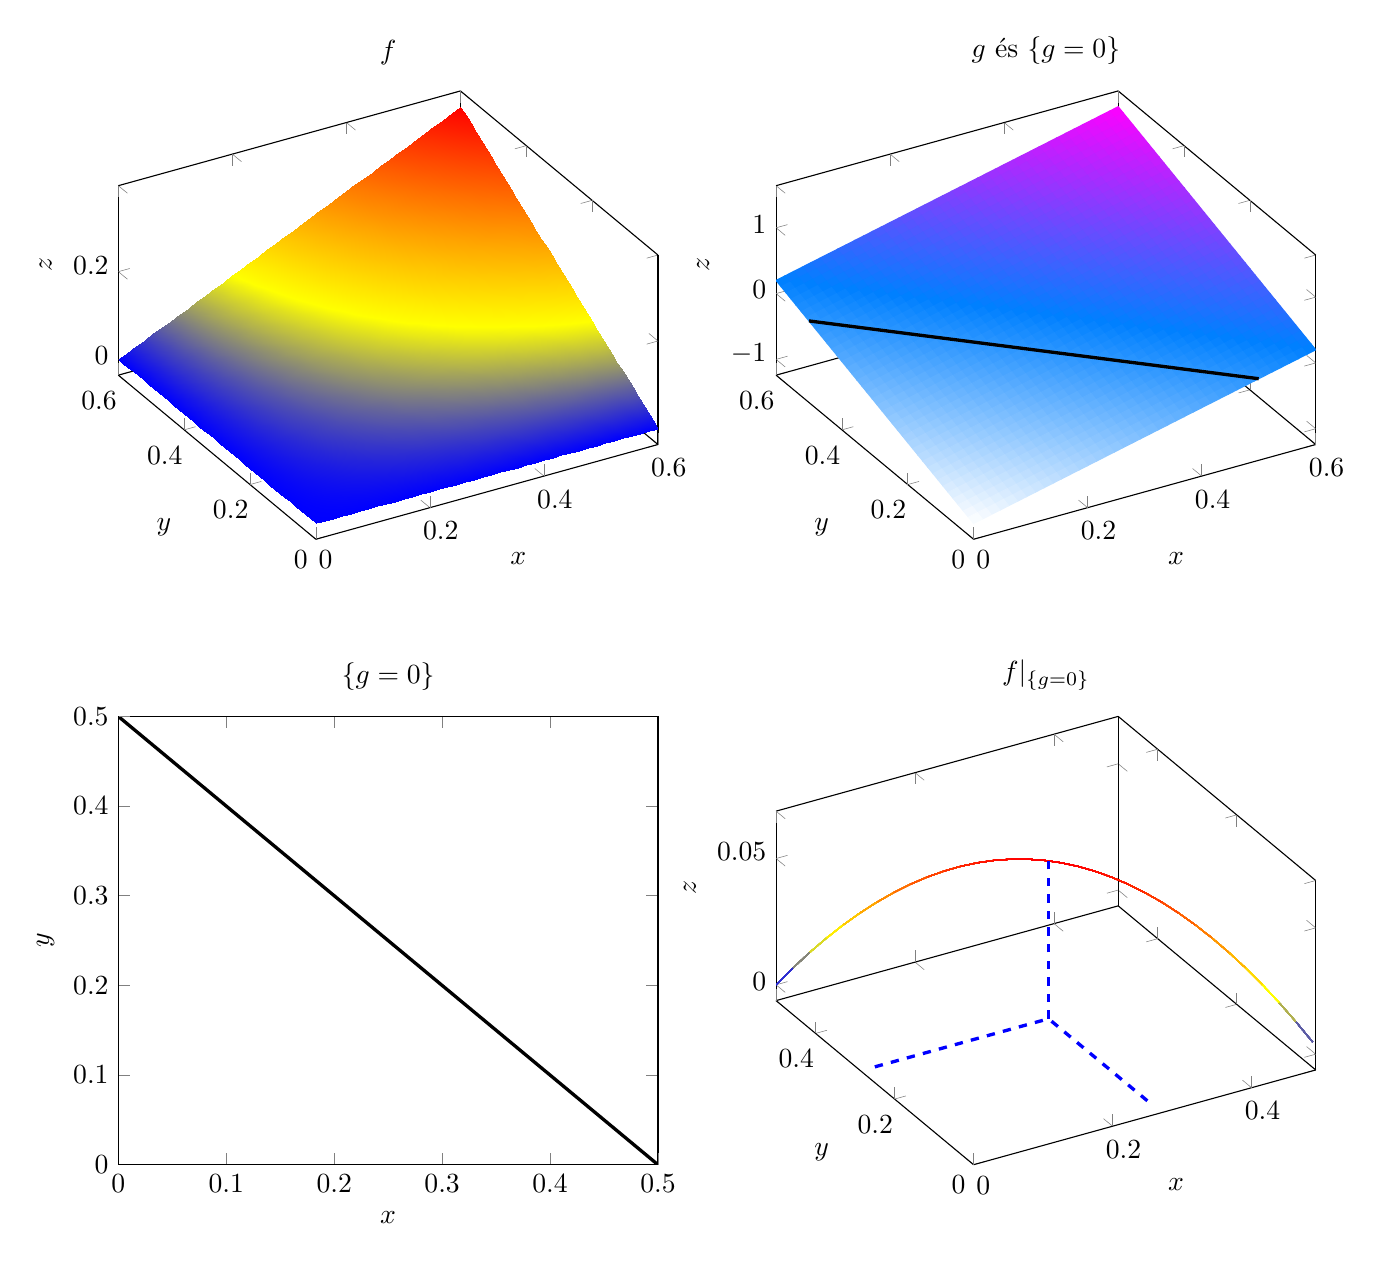
\begin{tikzpicture}
\begin{groupplot}[
        group style={
            group size=2 by 2,
            horizontal sep=1.5cm,
            vertical sep=2.25cm
        },
        view={-30}{45},
        domain=0:0.6,
        samples=40,
        shader=flat,
        xlabel={$x$}, ylabel={$y$}, zlabel={$z$},
        scaled ticks=false,
        tick label style={/pgf/number format/fixed}
    ]

    \nextgroupplot[title={$f$}, shader=interp]

    \addplot3[
        surf,
        colormap/hot
    ]
    {x * y};

    \nextgroupplot[title={$g$ és $\{g=0\}$}]

    \addplot3[
        surf,
        colormap/cool
    ]
    {2*x + 2*y - 1};

    \addplot3[
        very thick,
        color=black,
        domain=0:0.5,
        y domain=0:0.5
    ]
    (x, {0.5 - x}, 0);

    \nextgroupplot[title={$\{g=0\}$}, view={0}{90}]

    \addplot3[
        very thick,
        color=black,
        domain=0:0.5
    ]
    (x, {0.5 - x}, 0);

    \nextgroupplot[title={$f|_{\{g=0\}}$}, view={-30}{45}]

    \addplot3[
        surf,
        colormap/hot,
        restrict z to domain=0:1
    ]
    (x, {0.5 - x}, {x*(0.5-x)});

    \addplot3[
        very thick,
        dashed,
        color=blue,
    ] coordinates {
        (0, 0.25, 0)
        (0.25, 0.25, 0)
    };
    
    \addplot3[
        very thick,
        dashed,
        color=blue,
    ] coordinates {
        (0.25, 0, 0)
        (0.25, 0.25, 0)
    };

    \addplot3[
        very thick,
        dashed,
        color=blue,
    ] coordinates {
        (0.25, 0.25, 0)
        (0.25, 0.25, 0.0625)
    };
\end{groupplot}
\end{tikzpicture}
\end{center}

\newpage

Látjuk, hogy $\displaystyle\mathcal D_{f|_{\{g=0\}}} = \{g=0\}$ halmaz egy egyenes pontjait írja le, így természetesen egyik pontja se lehet belső pont, azaz tényleg nem alkalmazhatóak az eddigi tételeink. Ettől függetlenül persze az $f|_{\{g=0\}}$ leszűkítésnek lehetnek szélsőértékei, ahogy azt az utolsó ábra is mutatja.

\textbf{Ötlet:} Vegyük a $h(x) := \frac 12 - x \quad (x \in \R)$ függvényt, ami a $\{g=0\}$ halmaz által leírt egyenes explicit alakja, vagyis $\graf h = \{g = 0\}$.

Ekkor $f|_{\{g=0\}}$ helyett vizsgálhatjuk a $\Phi : \R \to \R,\ \Phi(x) := f(x,h(x)) = x(\frac 12 - x) \ (x \in \R)$ függvényt. Vegyük észre, hogy $\mathcal D_\Phi = \R$ minden pontja belső pont, azaz probléma nélkül alkalmazhatóak rá a lokális szélsőértékre vonatkozó szükséges és elégséges feltételek tételei.

$\Phi'(x) = \frac 12 - 2x = 0 \Longleftrightarrow x = \frac 14 \implies y = (\frac 12 - x) = \frac 14$ és $\Phi''(x) = -2 < 0\implies$ maximum.

Tehát az egységkerületű téglalapok közül az $x=y=\frac14$ oldalhosszú négyzet lesz a maximális területű.

\begin{center}
    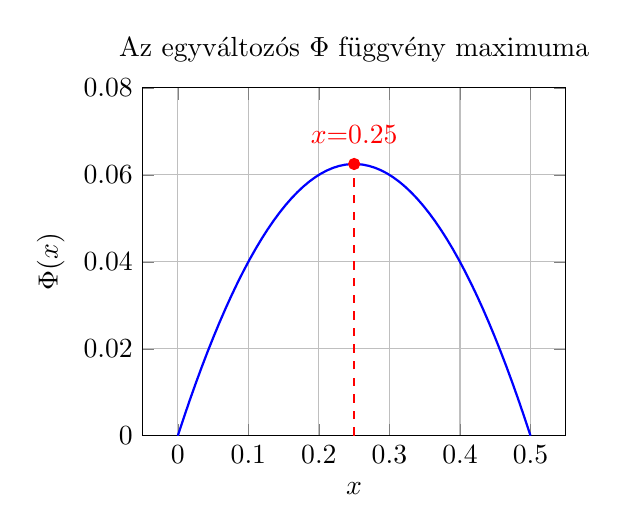
\begin{tikzpicture}
        \begin{axis}[
            title={Az egyváltozós $\Phi$ függvény maximuma},
            scaled ticks=false,
            tick label style={/pgf/number format/fixed},
            xlabel={$x$},
            ylabel={$\Phi(x)$},
            height=6cm,
            grid=major,
            ymin=0,
            ymax=0.08
        ]

        \addplot[blue, thick, domain=0:0.5, samples=60] {x*(0.5-x)};
        \addplot[red, dashed, thick] coordinates {(0.25,0) (0.25, 0.0625)};
        \addplot[only marks, mark=*, red] coordinates {(0.25, 0.0625)};
        \node[red, above] at (axis cs:0.25,0.065) {$x$=0.25};
            
        \end{axis}
    \end{tikzpicture}
\end{center}

\emph{Nagyon} informálisan nézve: itt azzal, hogy az $f$ függvény egyik változóját a másikból ki tudtuk fejezni (persze csak a leszűkítésen!), kvázi ``elcsaltunk'' egy dimenziót. A maradék dimenziónkban pedig tökéletesen tudunk mozogni minden irányba, kb. ``hozzáillesztve'' az ``elcsalt'' dimenzió-beli pozíciónkat. A fő különbség, hogy itt már nem tárol el az egyik függvény változó ``felesleges'' információt, azaz a belső pont megkötés élesedik arra az egy változónkra, ami az összes információt tartalmazza. Ez ellentétben áll az eredeti felállással, ahol azt vártuk volna el, hogy két, ``közös információt'' is tartalmazó, változó külön-külön is szabadon mozgatásával a halmazon belül maradjunk. A $h$ függvény bevezetésével ez megoldódik, mivel $\Phi$-ben a $h$ segítségével mi adjuk meg, hogy az egy változónk elmozgatása szerint a másikat hogyan kell módosítani (tulajdonképpen a ``közös információ'' alapján).

A fenti feladat ezzel az intuícióval több változóra is kiáltalánosítható, a feltételes szélsőérték (és később az implicitfüggvény) fogalmának bevezetésével.

\subsection{Definíció}

Legyen $1 \le n, m \in \N,\ \emptyset \ne U \subset \R^n$ és $f : U \to \R, g = (g_1,\,\ldots,\, g_m) : U \to \R^m$.

Ekkor $f$ függvénynek a \textbf{$g = 0$ feltételre vonatkozóan feltételes lokális maximuma (minimuma) van a $c \in \{g = 0\} := \{\xi \in U : g(\xi) = 0\}$ pontban}, ha az $\tilde f(\xi) := f(\xi)\quad (\xi \in \{g=0\})$ függvénynek $c$-ben lokális maximuma (minimuma) van.

Továbbá elnevezzük $f(c)$-t \textbf{feltételes lokális maximum (minimum)} vagy \textbf{szélsőérték}nek, és $c$-t pedig \textbf{feltételes lokális maximumhely (minimumhely)} vagy \textbf{szélsőértékhely}nek.

\subsubsection{Megjegyzések}

Feltesszük továbbá, hogy $\{g=0\} \ne \emptyset$,

A definícióban szereplő $\tilde f(\xi)$ az $f|_{\{g=0\}}$ leszűkítés.

\begin{samepage}
Tehát, ha $f$-nek egy $c \in \{g=0\}$ pontban lokális szélsőértéke van a $g=0$ feltételre nézve, akkor $\exists K(c)$, amire maximumnál $f(\xi) \le f(c)$, minimumnál $f(\xi) \ge f(c) \quad (\xi \in \{g=0\}\cap K(c))$.
\end{samepage}

\section{Feltételek}

\subsection{Elsőrendű szükséges feltétel}

\subsubsection{Tétel}

Legyen $1 \le n,m \in \N,\ m < n,\ \emptyset \ne U \subset \R^n$ nyílt és $f : U \to \R,\ g = (g_1,\,\ldots,\,g_m) : U \to \R^m$.

Továbbá tegyük fel, hogy

\begin{enumerate}[label=(\alph*),itemsep=1pt,topsep=1pt]
    \item $f \in D$
    \item $g \in C^1$
    \item $f$-nek $c\in\{g=0\}$ helyen feltételes lokális szélsőértéke van $g=0$ feltételre nézve
    \item $g'(c)$ Jacobi-mátrix rangja egyenlő $m$-mel
    ($\Leftrightarrow$ a gradiensvektorok lineárisan függetlenek),
    azaz $\rang g'(c) = m$. Ezt hívjuk \emph{rangfeltételnek}.
\end{enumerate}

Ekkor $\exists \lambda \in \R^m : \grad (f + \lambda g)(c) = 0$, ahol $\displaystyle(\lambda g)(\xi) := \dprod {\lambda,g(\xi)} = \sum_{i=1}^m \lambda_ig_i(\xi) \quad (\xi \in U)$.

Vegyük észre, hogy a tétel nagyon hasonló a feltétel nélküli esethez, csak itt a vizsgált $f$ függvény helyett az $f_\lambda := f + \lambda g$ függvényre vonatkozik. A $\lambda_i$-ket \textbf{Lagrange-multiplikátor} nevezzük, $f_\lambda$-t pedig \textbf{Lagrange-függvénynek}.  Hasonlóan fog felépülni a következő két tétel is.

\subsection{Másodrendű elégséges feltétel}

\subsubsection{Feltételes definitség}

A tétel kimondása előtt be kell vezetnünk a feltételes definitség fogalmát.

Legyen $Q : \R^n \to \R$ egy kvadratikus alak és $B \in \R^{m\times n}$. Vegyük az $\mathcal A_B := \{x \in \R^n : B\cdot x = 0\}$ halmazt.
Továbbá tfh. $m < n$ és $\rang B = m$.

Ekkor a $Q$ kvadratikus alak $B$-re nézve:
\begin{enumerate}[label=(\alph*),itemsep=1pt,topsep=1pt]
    \item \textbf{feltételesen pozitív definit}, ha $Q(x) > 0 \quad (0 \ne x \in \mathcal A_B)$
    \item \textbf{feltételesen negatív definit}, ha $Q(x) < 0 \quad (0 \ne x \in \mathcal A_B)$
    \item \textbf{feltételesen pozitív szemidefinit}, ha $Q(x) \ge 0 \quad (x \in \mathcal A_B)$
    \item \textbf{feltételesen negatív szemidefinit}, ha $Q(x) \le 0 \quad (x \in \mathcal A_B)$
\end{enumerate}

\subsubsection{Tétel}

\begin{samepage}

Legyen $1 \le n,m \in \N,\, m < n,\, \emptyset \ne U \subset \R^n$ nyílt és $f : U \to \R,\ g : U \to \R^n$. 
    
Továbbá tegyük fel, hogy
\begin{enumerate}[label=(\alph*), itemsep=1pt, topsep=1pt]
    \item $f,\,g \in D^2$
    \item $c \in \{g=0\}$-ben $\rang g'(c) = m$
    \item egy $\lambda \in \R^m$ vektorral vett $f_\lambda := f + \lambda g$-re:
    \begin{enumerate}[label=(\roman*),itemsep=1pt,topsep=1pt]
        \item $\grad f_\lambda(c) = 0$
        \item $Q_c^{f_\lambda}$ kvadratikus alak a $g'(c)$ mátrixra nézve feltételesen pozitív (negatív) definit
    \end{enumerate}
\end{enumerate}

Ekkor $f$-nek $c$-ben a $g=0$ feltételre vonatkozóan feltételes lokális minimuma (maximuma) van.

\end{samepage}

\subsection{Másodrendű szükséges feltétel}

\subsubsection{Tétel}

Legyen $1 \le n,m \in \N,\, m < n,\, \emptyset \ne U \subset \R^n$ nyílt, $f : U \to \R,\, g: U \to \R^m$ és $c \in \{g=0\}$.

Továbbá tegyük fel, hogy
\begin{enumerate}[label=(\alph*), itemsep=1pt, topsep=1pt]
    \item $f,\,g \in D^2$
    \item $\rang g'(c) = m$
    \item $f$-nek $c$-ben a $g=0$ feltételre vonatkozóan feltételes lokális minimuma (maximuma) van
\end{enumerate}

Ekkor $\exists \lambda \in \R^m$, amivel $f_\lambda := f + \lambda g$-re teljesül, hogy

\begin{enumerate}[label=(\alph*), itemsep=1pt, topsep=1pt]
    \item $\grad f_\lambda(c) = 0$
    \item $Q_c^{f_\lambda}$ kvadratikus alak $g'(c)$ mátrixra nézve feltételesen pozitív (negatív) szemidefinit
\end{enumerate}

\needspace{7\baselineskip}
\subsection{Megjegyzések}

\subsubsection{$m = n$ eset}

A feltételeknél $m < n$ feltevéssel éltünk, azonban könnyen belátható, hogy $m = n$ esetén is működnek az állítások. Nézzük például az elsőrendű szükséges feltételt.

\begin{samepage}
Ilyenkor $g'(c) \in \R^{n \times n}$ és a $\rang g'(c) = m = n$ rangfeltétel miatt a
$$
g'(c) = 
\begin{bmatrix}
\grad g_1(a) \\
\vdots \\
\grad g_n(a)
\end{bmatrix}
\in \R^{n \times n}
$$
Jacobi-mátrix \emph{invertálható.}
\end{samepage}

Vagyis a $\grad g_k(a) \in \R^n \ (k = 1,\ldots,n)$ vektorok lineárisan függetlenek, azaz bázist alkotnak $\R^n$-ben. Így bármilyen $\R^n$-beli vektor előállítható a lineáris kombinációjukként, spec.:
$$\exists! \lambda_j \in \R \enspace (j = 1,\ldots, n) : \sum_{j=1}^n \lambda_j \grad g_j(c) = -\grad f(c)$$

Tehát a $\lambda := (\lambda_1, \ldots, \lambda_n) \in \R^n$ vektorral teljesül, hogy $\grad (f + \lambda g)(c) = 0$. Ez alapján $n = m$ esetben is teljesül a tétel, azonban ott triviális.

\subsubsection{$\lambda$ és $c$ értékek meghatározása}

Szeretnénk felírni egy egyenletrendszert, amiből meghatározhatjuk a $\lambda_1,\ldots,\lambda_m$ és $c_1,\ldots,c_n$ értékeket. Ehhez $n + m$ darab egyenlet fog kelleni.

Vegyük az $\displaystyle f_\lambda := f + \lambda g = f + \sum_{k=1}^m \lambda_k \cdot g_k$ függvényt.

Az elsőrendű szükséges feltétel szerint $\grad f_\lambda(c) = 0$, amit ha kibontunk:

$$\partial_j f(c_1,\ldots,c_n) + \sum_{k=1}^m\lambda_k \partial_j g_k(c_1,\ldots,c_n)=0 \quad (j = 1,\ldots, n)$$

Ez összesen $n$ darab egyenletet fog adni. A maradék $m$ egyenletet a $g(c)=0$ feltételből kapjuk, ugyanis $g_l(c_1, \ldots,c_n) = 0 \quad (l = 1,\ldots,m)$.

\subsubsection{$\R^2$-beli feltételes definitség $g'(c)$-re nézve}\label{note:cond-orto}

Nézzük a $B := g'(c) \in \R^{m \times n}$, $m$-rangú mátrixszal vett $\mathcal A_B := \{y \in \R^n : B \cdot y = 0\}$ halmazt $m=1,\ n=2$ esetben:

Ekkor $0 \ne B = \grad g(c) \in \R^2$ és $\mathcal A_B = \{y \in \R^2 : \dprod{\grad g(c),\,y} = 0\}$.

Skaláris szorzat tulajdonságai alapján ekkor tudjuk, hogy $x \in \mathcal A_B$ azzal ekvivalens, hogy $x$ merőleges a gradiensre. Vagyis az $\mathcal A_B$ halmaz az origón átmenő, $\grad g(c)$ vektorra merőleges egyenes.

Hasonlóan $m=1,\, n > 2$ esetben pedig $\grad g(c)$ és $x$ ortogonálisak kell, hogy legyenek.

\subsubsection{Példafeladat}

Legyen $n := 2,\, m:=1,\,f(x,y) := 2x + 3y$ és $g(x,y) := x^2+y^2-1 \enspace \big((x,y) \in \R^2\big)$.

Ezek alapján definiáljuk $f_\lambda$-t: $f_\lambda(x,y) := 2x + 3y + \lambda(x^2+y^2-1) \enspace \big((x,y) \in \R^2\big)$.

Ekkor az elsőrendű szükséges feltétel szerint a következő egyenletrendszer megoldásaiban lehet csak feltételes lokális szélsőértéke a függvénynek $g = 0$ feltételre nézve:
\begin{alignat*}{2}
    \partial_1 f_\lambda(x,y) &= 2 + 2\lambda x &&= 0 \\
    \partial_2 f_\lambda(x,y) &= 3 + 2\lambda y &&= 0 \\
    g(x,y)                    &= x^2 + y^2 - 1  &&= 0
\end{alignat*}

Számoljuk ki az egyenletrendszer megoldásait:
\begin{gather*}
    x_1 := \frac 2 {\sqrt{13}},\ y_1 := \frac 3 {\sqrt{13}},\ \lambda_1 := -\frac {\sqrt{13}} 2,
    \\
    x_2 := -\frac 2 {\sqrt{13}},\ y_2 :=  -\frac 3 {\sqrt{13}},\ \lambda_2 := \frac {\sqrt{13}} 2
\end{gather*}

Ezekre teljesül, hogy $g'(x_i, y_i) = \grad g(x_i, y_i) = (2x_i, 2y_i) = 2(x_i, y_i) \quad (i = 1,2)$.

Valamint a $c^{(i)} := (x_i, y_i) \in \R^2 \enspace (i = 1,2)$ jelölés bevezetésével:
$$Q_{c^{(i)}}^{f_\lambda}(x,y) =
\dprod{
    \begin{bmatrix}
        2\lambda_i & 0 \\
        0 & 2\lambda_i
    \end{bmatrix}
    \cdot
    \xymat
,\, \xymat}
=
\dprod{
    \begin{bmatrix}
        2\lambda_ix \\
        2\lambda_iy
    \end{bmatrix},
    \xymat
}
=
2 \lambda_i(x^2 + y^2)$$

\begin{gather*}
Q_{c^{(1)}}^{f_\lambda}(x,y) = -\sqrt{13}(x^2+y^2) < 0
\enspace \text{és} \enspace
Q_{c^{(2)}}^{f_\lambda}(x,y) = \sqrt{13}(x^2+y^2) > 0
\\[4pt]
\big((x,y) \in \R^2 \setminus \{(0,0)\}\big)
\end{gather*}

Tehát $Q_{c^{(1)}}^{f_\lambda}$ negatív definit, $Q_{c^{(2)}}^{f_\lambda}$ pozitív definit, vagyis a másodrendű elégséges feltétel szerint $f$-nek $c^{(1)}$-ben feltételes lokális maximuma, $c^{(2)}$-ben feltételes lokális minimuma van.

\section{Elsőrendű szükséges feltétel bizonyítása}

\subsection{Tétel}

Legyen $1 \le n,m \in \N,\ m < n,\ \emptyset \ne U \subset \R^n$ nyílt és $f : U \to \R,\ g = (g_1,\,\ldots,\,g_m) : U \to \R^m$.

Továbbá tegyük fel, hogy
\begin{enumerate}[label=(\alph*),itemsep=1pt,topsep=1pt]
    \item $f \in D$
    \item $g \in C^1$
    \item $f$-nek $c\in\{g=0\}$ helyen feltételes lokális szélsőértéke van $g=0$ feltételre nézve
    \item $\rang g'(c) = m$
\end{enumerate}
Ekkor $\exists \lambda \in \R^m : \grad (f + \lambda g)(c) = 0$, ahol $\displaystyle(\lambda g)(\xi) := \dprod {\lambda,g(\xi)} = \sum_{i=1}^m \lambda_ig_i(\xi) \quad (\xi \in U)$.
\vspace{-18pt}
\subsection{Bizonyítás}

Egy gyors lebontása a ``szereplőinknek'', támpontnak a bizonyítás során:
\begin{itemize}[itemsep=1pt,topsep=1pt]
    \item $m < n$
    \item $U \subset \R^n$ nyílt
    \item $f : U \to \R$ (azaz $f \in \R^n \to \R$) és $f \in D$
    \item $g : U \to \R^m$ (azaz $g \in \R^n \to \R^m$) és $g \in C^1$
    \item $\{g=0\} \subset U \subset \R^n$
    \item $c \in \{g=0\}$, vagyis $c \in \R^n$
    \item $\rang g'(c) = m$
\end{itemize}

\subsubsection{Bizonyítás}

A rangfeltételből tudjuk, hogy $g'(c) \in \R^{m\times n}$ mátrixnak létezik $A \in \R^{m \times m}$ részmátrixa, amire $\det A \ne 0$ (mivel az összes ($m$ darab) sora lineárisan független). 

Jelöljük az $A$ mátrixot meghatározó oszlopok indexét $j_1, \ldots, j_m$-el, majd vegyük a következő indexhalmazt:
$$\{i_1, \ldots, i_{n-m}\} := \{1, \ldots, n\} \setminus \{j_1, \ldots, j_m\}$$
Ekkor $j_k \enspace (k = 1,\ldots,m)$ a lineárisan független oszlopokat indexeli, $i_k \enspace (k = 1,\ldots,n-m)$ pedig a maradékot.

Ha nehézséget okoz a bizonyítás megértése, vagy inkább az intuíció az egész mögött, akkor egy rövid, megértést remélhetőleg segítő szekció megtalálható a függelékben (ld. \ref{sec:cond-expl}), azonban ott használva vannak az eddig bevezetett jelölések.

\bigskip

Vezessük be eszerint az $\R^n \equiv \R^{n-m} \times \R^m$ felbontást, azaz
\begin{gather*}
    \xi = (\xi_1, \ldots, \xi_n) = (x,y) \in \R^n, \enspace \text{ahol} \\
    x := (\xi_{i_1},\ldots,\xi_{i_{n-m}}) \in \R^{n-m},\ y := (\xi_{j_1},\ldots,\xi_{j_m}) \in \R^m
\end{gather*}

Tehát tulajdonképpen itt az indexek által megadott permutáció szerint átrendeztük a mátrix oszlopait úgy, hogy $y$-ba kerüljenek a lineárisan független oszlopok, $x$-be pedig a maradék.\footnote{Belátható, hogy ez a permutáció nem lesz hatással semmilyen számunkra fontos tulajdonságra nézve. Ez az $i$ és $j$ szerinti indexelés a könyvből származik, a segédanyag egyszerűen felteszi, hogy $A$ az utolsó $m$ oszlopában áll elő $g'(c)$-nek, ekkor $x = (\xi_1,\ldots,\xi_{n-m}),\ y = (\xi_{n-m+1},\ldots,\xi_n)$. Vizsgán ennek is egy teljesen elfogadott módszernek kell lennie, persze indoklásnak kellhet, hogy meg tudunk adni egy $\sigma$ permutációt, ami ezt előállítja, majd a végén alkalmazni tudjuk $\sigma^{-1}$-t a tulajdonságok sérülése nélkül.}
% TODO: levezetés, hogy miért nem sérülnek a tulajdonságok?

Szedjük szét a felbontás szerint $c$-t is, $c = (a,b)$ komponensekre. Ekkor $\partial_2 g(a,b) = A$, amiről tudjuk, hogy invertálható, vagyis $\det \partial_2 g(a,b) \ne 0$ következik. Továbbá $c \in \{g=0\}$ miatt $g(a,b) = 0$, így alkalmazhatjuk az implicitfüggvény-tételt.

Ekkor alkalmas $K(a) \subset \R^{n-m},\ K(b) \subset \R^m$ környezetekkel létezik $g$ által az $(a,b)$ körül meghatározott $h : K(a) \to K(b)$ implicitfüggvény, amire $h \in C^1$ és
$$h'(x) = -\Big(\partial_2g(x,h(x))\Big)^{-1} \cdot \partial_1g(x,h(x)) \quad (x \in K(a))$$

Világos\footnote{
Annyira nem, tekintve hogy ez az állítás egyáltalán nem tartja tiszteletben a fenti permutációnkat, de nem aggódunk túlságosan emiatt, mivel a könyv se aggódott túlságosan emiatt.
}, hogy ha a $\{g=0\}$ halmazt leszűkítjük ezekre a környezetekre, akkor
$$\big(K(a) \times K(b)\big)\cap \{g=0\} = \{(x,\,h(x)) \in U : x \in K(a)\}$$

Mivel $c$ feltételes lokális szélsőértéke $f$-nek $g=0$-ra nézve, így $f(\xi) \le f(c) \enspace (\xi \in K(c) \cap \{g=0\})$.\footnote{
Itt most feltettük, hogy $f(c)$ feltételes lokális maximum. Minimumra természetesen ezzel analóg módon történik a levezetés.
}

Feltehető $K(a) \times K(b) \subset K(c)$.

Definiáljuk a $\Phi(x) := f(x,\, h(x)) \enspace (x \in K(a))$ függvényt, amire $\Phi(x) \le f(c) = \Phi(a)$ teljesül, bármely $x \in K(a)$ mellett. Tehát $\Phi$-nek lokális maximuma van $a$-ban. 

Mivel $\Phi \in D(K(a))$ is teljesül, így
$$\Phi'(a) = \grad \Phi(a) = 0$$

Vezessük be a $\varphi(x) := (x, h(x)) \enspace (x \in K(a))$ függvényt, amivel $\Phi = f \circ \varphi$. Teljesül továbbá $\varphi \in D$, valamint ha $I$ az $\R^{(n-m)\times(n-m)}$ egységmátrixot jelöli, akkor
$$\varphi'(x) = \begin{bmatrix}I \\ h'(x)\end{bmatrix} \in \R^{n\times(n-m)}\qquad (x \in K(a))$$

A fentiek, és az összetett függvények deriváltja tétel alapján,

\begin{gather*}
    0 = \Phi'(a) = f'(\varphi(a)) \cdot \varphi'(a) = f'(a,h(a)) \cdot \begin{bmatrix}I \\ h'(a)\end{bmatrix} = f'(c) \cdot \begin{bmatrix}I \\ h'(a)\end{bmatrix} = \\
    \partial_1f(c) + \partial_2f(c)\cdot h'(a) = \partial_1f(c) - \partial_2f(c) \cdot \big(\partial_2g(c)\big)^{-1}
\cdot \partial_1g(c)\end{gather*}

Ekkor legyen $\lambda := -\partial_2f(c)\cdot\big(\partial_2g(c)\big)^{-1} \in \R^m$, ezzel $0 = \partial_1 f(c) + \lambda\cdot\partial_1g(c)$.

Továbbá $\big(\partial_2g(c)\big)^{-1}$-el ``átszorozva'' kapjuk, hogy: $\partial_2f(c) + \lambda \cdot \partial_2g(c) = 0$.

Ebből a $\partial_1$ és $\partial_2$ tagokat kibontva kapjuk a következő egyenlőségeket:
\begin{align*}
\partial_{i_k}f(c) + \sum_{l=1}^m \lambda_l\cdot\partial_{i_k}g_l(c) &= 0 \quad (k=1,\ldots,n-m) \\
\partial_{j_k}f(c) + \sum_{l=1}^m \lambda_l \cdot \partial_{j_k}g_l(c) &= 0 \quad (k=1,\ldots,m)
\end{align*}

Ezeket összevonva pedig:
$$\partial_k f(c) + \sum_{l=1}^m \lambda_l \cdot \partial_kg_l(c) = 0 \quad (k = 1,\ldots,n)$$

Tehát $\displaystyle \grad (f + \lambda g)(c) = \left( \partial_1f(c) + \sum_{l=1}^m \lambda_l \cdot \partial_1g_l(c), \ldots, \partial_n f(c) + \sum_{l=1}^m \lambda_l \cdot \partial_n g_l(c) \right) = 0$. \qed
\chapter{*Differenciálegyenletek alapjai}

\setcounter{footnote}{0}

\section{Követelmények}
\begin{enumerate}
    \item Differenciálegyenlet (rendszer) fogalma, kezdetiérték-probléma (Cauchy-feladat)
    \item Egzakt egyenlet
    \item Szeparábilis egyenlet
    \item Rakéta emelkedési idejének kiszámítása
\end{enumerate}

\section{Differenciálegyenletek}

\begin{definition}[differenciálegyenlet]\label{def:de}
Legyen $1 \le n \in \N$ és $I \subset \R$ és $\Omega \subset \R^n$ nyílt intervallumok.\footnote{
Itt mondhatnánk, hogy $\Omega$ szempontjából elég azokkal az esetekkel foglalkozni, ahol egy kicsit szigorúbb feltételt teljesít: $\Omega$ egy $\R^n$-beli tartomány. Azonban azt megadni, hogy ez mit is jelent, új topológiai fogalmakat használna, ezért ezt a segédanyag is mellőzi. A könyv azonban részletesebb kifejti ezeket, így ha lesz rá időm, készítek neki egy bekezdést a függelékben. % TODO
} Tegyük fel, hogy az $f : I \times \Omega \to \R^n$ függvényre $f \in C$ teljesül.
Ekkor a feladat:

Határozzunk meg olyan $\varphi \in I \to \Omega$ függvényt, amire
\begin{enumerate}[label=(\alph*),itemsep=1pt,topsep=1pt]
    \item $\dom_\varphi$ nyílt intervallum
    \item $\varphi \in D$
    \item $\varphi'(x) = f(x,\,\varphi(x)) \quad (x \in \dom_\varphi)$
\end{enumerate}

Ezt a feladatot hívjuk \textbf{explicit elsőrendű közönséges differenciálegyenletnek} (röviden \textbf{differenciálegyenletnek}), és bevezetjük rá a \emph{d.e.} rövidítést.
\end{definition}

\begin{remarks}
\
\begin{enumerate}[label=\roman*),itemsep=1pt]
    \item Minden, a fenti feltételeket kielégítő $\varphi$ függvény a d.e. \textbf{megoldása}.
    \item Az $f$ függvény pedig a d.e. \textbf{jobb oldala}.
    \item Ha $\varphi$ egy megoldás, minden $J \subset \dom_\varphi$ nyílt intervallumon vett $\restrict \varphi J$ leszűkítés is megoldás.
    \item Az $\R \times \R^n \equiv \R^{n+1}$ azonosítás miatt az $f$ mint egy $\R^{n+1} \to \R^n$ leképezés, azaz $n+1$ változós vektorfüggvényként is felfogható, mivel $I \times \Omega \subset \R^{n+1}$.
    \item Az elnevezésben a \emph{közönséges} azt jelenti, hogy egyváltozós függvényt keresünk (nincsenek parciális deriváltak), az \emph{elsőrendű} azt, hogy nincsen elsőnél magasabb rendű deriváltra feltételünk, az \emph{explicit} pedig azt, hogy a deriváltra nézve van kifejezve a feltétel.
    \item Az \emph{implicit} alaknál $f$ helyett veszünk pl. egy $F : I \times \Omega \times \R^n \to \R^n,\ F \in C$ függvényt és $F(x,\,\varphi(x),\,\varphi'(x))=0$ formában adjuk meg a feltételt.
\end{enumerate}

\end{remarks}

\begin{definition}[kezdetiérték-probléma]
Ha adott $\tau \in I,\ \xi \in \Omega$ mellett kikötjük még $\tau \in \dom_\varphi$ és $\varphi(\tau) = \xi$ feltételeket is, akkor \textbf{kezdetiérték-problémának} hívjuk a feladatot (vagy \textbf{Cauchy-feladatnak}), és \emph{k.é.p.}-nek rövidítjük.
\end{definition}

\begin{definition}[differenciálegyenlet rendszer]
A \ref{def:de} definícióban legyen $n \ge 2$.

Ekkor $\varphi = (\varphi_1, \ldots, \varphi_n)$ és $f = (f_1, \ldots, f_n)$.
$$\varphi'(x) = f(x, \varphi(x)) \eqv \varphi_i'(x) = f_i(x, f_1(x), f_2(x), \ldots, f_n(x)) \quad (x \in \dom_\varphi)$$

Ilyenkor \textbf{differenciálegyenlet rendszerről} beszélünk, \emph{d.e.r.}-nek rövidítjük.

Tehát a differenciálegyenlet rendszerek a differenciálegyenlet feladat $n \ge 2$ esetei.
\end{definition}

\subsection{Teljes megoldás}

\subsubsection{Felvezető példa}

A \ref{def:de} definícióban legyen $n := 1,\ I := \Omega := \R$. Vizsgáljuk ekkor az $f(x,y) := \sqrt{|y|} \quad \big((x,y) \in \R\big)$ jobb oldallal rendelkező $\tau := \xi := 0$ k.é.p.-et.

Olyan nyílt $\dom_\varphi$ intervallumon értelmezett $\varphi \in \R \to \R$ függvényt keresünk tehát, amire $\varphi \in D$ teljesül, $\varphi(0) = 0$, és
$$\varphi'(x) = f(x,\varphi(x)) = \sqrt{|\varphi(x)|} \quad \big((x,y) \in \dom_\varphi\big)$$

Ekkor $\varphi \equiv 0$ egy megoldása a differenciálegyenletnek.

De ugyanakkor a következő, lényegesen különböző $\tilde\varphi$ függvény is:
$$\tilde\varphi(x) := \begin{cases}
    \dfrac {x^2} 4 & (x \ge 0) \\[8pt]
    -\dfrac {x^2} 4 & (x < 0)
\end{cases}$$

Tehát a fenti k.é.p. nem oldható meg egyértelműen.

\begin{definition}[teljes megoldás]
Egy kezdetiérték-probléma \textbf{egyértelműen oldható meg}, ha tetszőleges $\varphi, \tilde\varphi$ megoldásokra
\begin{equation}\label{eq:kep-uni-sol-eqv}
\varphi(x) = \tilde\varphi(x) \qquad (x \in \dom_\varphi \cap \dom_{\tilde\varphi}).
\end{equation}

Legyen ekkor $\mathcal M$ a k.é.p. megoldásainak halmaza és
\vspace{-3pt}
$$J := \bigcup_{\varphi \in \mathcal M}\dom_\varphi$$

Ekkor $J\ (\subset I)$ nyílt\footnote{Ld. \emph{Analízis III., nyílt halmazok uniója}.}, valamint a $\tau \in \dom_\varphi$ k.é.p. feltétel és \eqref{eq:kep-uni-sol-eqv} miatt $\tau \in J$ is teljesül.

Legyen $\Phi : J \to \R : \Phi(x) := \varphi(x) \enspace (x \in J, \varphi \in \mathcal M)$. Ez tetszőleges $\varphi$-vel megadható \eqref{eq:kep-uni-sol-eqv} miatt.

Ekkor szintén \eqref{eq:kep-uni-sol-eqv} és a k.é.p. feltételei szerint $\Phi(\tau) = \xi,\ \Phi \in D,$ és $\Phi'(x) = f(x,\Phi(x)) \enspace (x \in J)$.

Vagyis $\Phi \in \mathcal M$ és minden $\varphi \in \mathcal M$-re $\varphi(x) = \Phi(x) \enspace (x \in \dom_\varphi) \eqv \varphi = \restrict \Phi {\dom_\varphi}$.

Tehát a k.é.p. bármely megoldása megadható $\Phi$ egy leszűkítéseként.

Ekkor a $\Phi$ függvényt a kezdetiérték-probléma \textbf{teljes megoldásának} nevezzük.
\end{definition}

\section{Szeparábilis differenciálegyenletek}

\begin{definition}[szeparábilis differenciálegyenlet]
Legyen $n := 1$ és $I,J \subset \R$ nyílt intervallumok. Legyen továbbá $g : I \to \R,\ h : J \to R \setminus \{0\}$, amikre $g, h \in C$.

Tekintsük ekkor a $f(x,y) := g(x) \cdot h(x) \quad \big((x,y) \in I  \times J\big)$ jobb oldallal rendelkező differenciálegyenletet. Ekkor olyan $\varphi \in I \to J$ megoldást keresünk, amire
\begin{equation}\label{eq:sep-de-def}
\varphi'(x) = g(x) \cdot h(\varphi(x)) \qquad (x \in \dom_\varphi)
\end{equation}

Az ilyen alakban megadható differenciálegyenlet feladatot hívjuk \textbf{szeparábilis differenciálegyenletnek} (vagy \textbf{szétválasztható változójú differenciálegyenletnek}).

Legyenek adottak $\tau \in I,\ \xi \in J$ számok, amikre $\tau \in \dom_\varphi$ és $\varphi(\tau) = \xi$.

Ekkor egy \emph{szeparábilis differenciálegyenletre vonatkozó kezdetiérték-problémával} van dolgunk.\footnote{Az egyszerűség kevéért a jegyzet során ezekre röviden csak \emph{szeparábilis k.é.p.}-ként hivatkozok, de ez nem egy formális fogalom. Hasonlóan az egzakt d.e.-re vonatkozó k.é.p.-ekre pedig egzakt k.é.p.-ként, és így tovább.}
\end{definition}

\begin{theorem}[szeparábilis k.é.p. megoldás egyértelműsége]\label{sec:sep-uni}
\

Tetszőleges szeparábilis differenciálegyenletre vonatkozó kezdetiérték-probléma egyértelműen megoldható, és minden $\psi, \varphi$ megoldásaira:
\[\varphi(x) = \psi(x) \qquad (\dom_\varphi \cap \dom_\psi)\]
\end{theorem}
\begin{proof}\footnote{A követelmények között nem szerepel expliciten ez a bizonyítás, de a rakéta feladatra, mint szeparábilis k.é.p.-re adott megoldása a segédanyagnak a bizonyítás során bevezetett jelölésekre és egyenlőségekre hivatkozik, így kidolgoztam.}
A definícióban szereplő szimbólumokat értelmezzük itt is ugyanúgy.

Mivel bármely $x \in J$-re $h(x) \ne 0$, egy $\varphi$ megoldással a \eqref{eq:sep-de-def} egyenlőség átrendezhető $g$-re, vagyis
\begin{equation}\label{eq:sep-uni-proof-start}
\frac {\varphi'(x)} {h(\varphi(x))} = g(x) \quad (x \in \dom_\varphi)
\end{equation}

ahol $\dom_\varphi \subset I$ nyílt intervallum.

Mivel $g$ és $\dfrac 1 h$ nyílt intervallumon értelmezett ($\dom_g = I$ és $\dom_{1/h}=J$), folytonos függvények, így megadható egy primitív függvényük, tehát
$$\exists G : I \to \R,\ H : J \to \R \text{ amikre } G,H \in D \text{ és } G' = g, H' = \frac 1 h$$

Az összetett függvények deriváltja ($(H \circ \varphi)'(x) = H'(\varphi(x)) \cdot \varphi'(x)$) alapján \eqref{eq:sep-uni-proof-start} azt jelenti, hogy
$$(H \circ \varphi)'(x) = \frac {\varphi'(x)}{h(\varphi(x))} = g(x) = G'(x) \quad (x \in \dom_{\varphi})$$

Vagyis valamilyen $c \in \R$-vel,
$$(H \circ \varphi - G)'(x) = 0 \implies (H \circ \varphi - G)(x) = c \qquad (x \in \dom_\varphi)$$

Ekkor spec. $x := \tau$ esetben $H(\varphi(\tau)) - G(\tau) = H(\xi) - G(\tau) = c$.
Tehát,
\begin{equation}\label{eq:sep-uni-proof-hg-cond}
H(\varphi(x)) - G(x) = H(\xi) - G(\tau) \qquad (x \in \dom_\varphi)
\end{equation}

Vagyis \emph{ha léteznek} megoldások, akkor a fenti egyenlőség teljesül rájuk. Lássuk be, hogy valóban mindig lesz megoldása a feladatnak.

\paragraph*{Létezés.}

Definiáljuk az $F : I \times J \to \R,\ F(x,y) := H(y) - G(x) - H(\xi) + G(\tau)$ függvényt. Erre $F \in C^1$ és $F(\tau, \xi) = 0$ teljesülnek. Továbbá
$$\partial_2F(\tau, \xi) = H'(\xi) = \dfrac 1 {h(\xi)} \ne 0$$

Tehát $F$-re alkalmazható az \emph{implicitfüggvény-tétel} a $(\tau, \xi)$ pontban.

A tétel alapján $\exists K(\tau),\,K(\xi),\, \varphi : K(\tau) \to K(\xi)$ implicitfüggvény, amire $\varphi \in C^1$ és
$$\varphi'(x) = -\frac{\partial_1 F(x,\,\varphi(x))}{\partial_2 F(x,\,\varphi(x))} = -\frac {-G'(x)} {H'(\varphi(x))} = g(x) \cdot h(\varphi(x)) \qquad (x \in K(\tau))$$

teljesülnek. Továbbá szintén a tétel miatt $\varphi(\tau) = \xi$.

Ekkor tehát $\varphi$ egy megoldás.\partqed

\vspace{-2pt}
\paragraph*{Egyértelműség.}

Emlékezzünk, hogy tetszőleges $\tilde\varphi$ megoldásnak teljesíteni kell a \eqref{eq:sep-uni-proof-hg-cond} feltételt, valamilyen $G = g'$ és $H' = \dfrac 1 h$ primitív függvényekre.

\emph{Ötlet:} Mivel a \eqref{eq:sep-uni-proof-hg-cond} feltételnek mindenképpen teljesülnie kell, lássuk be, hogy az összes ilyen primitív függvény $\varphi$-hez fog vezetni.

Tegyük fel, hogy $\tilde H, \tilde G$ is megfelelő primitív függvények és $\tilde \varphi : \tilde K(\tau) \to \tilde K(\xi)$ egy megoldás, amire
$$\tilde H(\tilde \varphi(x)) - \tilde G(x) = \tilde H(\xi) - \tilde G(\tau) \qquad (x \in \dom_{\tilde\varphi})$$

Viszont $\exists \alpha, \beta \in \R : \tilde H = H + \alpha,\ \tilde G = G + \beta$.\footnote{
Ld. \emph{Analízis II., Primitív függvények (alap)tulajdonságai}
}
Tehát bármely $x \in \dom_{\tilde\varphi}$-re,
\begin{align}
H(\tilde\varphi(x)) + \alpha - G(x) - \beta &= H(\xi) + \alpha - G(\tau) - \beta \label{eq:sep-uni-wincon} \\
H(\tilde\varphi(x)) - G(x) &= H(\xi) - G(\tau) \notag
\end{align}

Tudjuk, hogy $H'(y) = \dfrac 1 {h(y)} \ne 0 \enspace (y \in J)$. Továbbá, mivel $H'$ egy deriváltfüggvény, így Darboux-tulajdonságú is.\footnote{
Ld. \emph{Analízis II., Darboux-tétel}
} Sőt, mivel nem veszi fel a $0$ értéket sehol, tudjuk, hogy állandó előjelű.\footnote{
Ui. a Darboux-tulajdonság (informálisan) azt garantálja, hogy a függvény bármely két értéke között felveszi az összes köztes értéket. Emiatt, ha előjelet váltana valahol $H'$, akkor fel kéne vennie ehhez a $0$-t is valahol.
} Ez alapján viszont $H$ szigorúan monoton\footnote{Ld. \emph{Analízis II., Monotonitás és derivált kapcsolata}}, és így invertálható is. Ekkor viszont \eqref{eq:sep-uni-proof-hg-cond} és \eqref{eq:sep-uni-wincon} egyenlőségek alapján:
\begin{alignat*}{4}
    & \varphi(x) && = H^{-1}(G(x) + H(\xi) - G(\tau)) \qquad && (x \in \dom_\varphi) \\
    & \tilde\varphi(x) && = H^{-1}(G(x) + H(\xi) - G(\tau)) \qquad && (x \in \dom_{\tilde\varphi}) \\
\implies & \varphi(x) && = \tilde\varphi(x) \qquad && (x \in \dom_\varphi \cap \dom_{\tilde\varphi})
\end{alignat*}

Tehát bármely $\tilde\varphi$ megoldás azonos lesz $\varphi$-vel $\dom_{\varphi} \cap \dom_{\tilde\varphi}$ leszűkítésen.
\end{proof}

\begin{remark}[Szeparábilis differenciálegyenlet megoldása integrálfüggvénnyel]
\

Vizsgáljuk meg a szeparábilis differenciálegyenletek megoldásában központi szerepet élvező \eqref{eq:sep-uni-proof-hg-cond} egyenlőséget. Ez átrendezhető a következő módon:
\begin{align*}
H(\varphi(x)) - G(x) &= H(\xi) - G(\tau) \qquad (x \in \dom_\varphi) \implies \tag{\ref{eq:sep-uni-proof-hg-cond}} \\
H(\varphi(x)) - H(\xi) &= G(x) - G(\tau) \qquad (x \in \dom_\varphi)
\end{align*}

Vegyük észre, hogy mivel $H,G$ primitív függvények, így ez a Newton-Leibniz tétel szerint felbontott alakja a következő integrálfüggvény egyenlőségnek:
\begin{equation*}
    \int^{\varphi(x)}_\xi \frac 1 {h(x)}\, dx = \int_\tau^x g(x)\,dx \qquad (x \in \dom_\varphi)
\end{equation*}

Vagyis általánosan a két integrál kiszámításával kapott egyenlőségből is megoldható a feladat.
\end{remark}

\section{Egzakt differenciálegyenletek}

\begin{definition}[egzakt differenciálegyenlet]
Legyenek $I, J \subset \R$ nyílt intervallumok és $g : I \times J \to \R,\ h : I \times J \to \R$ olyan függvények, amire $g,h \in C$, valamint $0 \notin \rng_h$. Olyan $\varphi : I \to J,\, \varphi \in D$ megoldást keresünk, amire $\dom_\varphi \subset I$ nyílt, és
$$\varphi'(x) = -\frac{g(x,\varphi(x))}{h(x,\varphi(x))} \qquad (x \in \dom_\varphi)$$

Egy így megfogalmazott feladat \textbf{egzakt differenciálegyenlet} akkor, \emph{ha}
$$I \times J \ni (x,y) \mapsto \big(g(x,y),\ h(x,y)\big) \in \R^2$$
leképezésnek van primitív függvénye.

Ez azt jelenti, hogy egy alkalmas $G : I \times J \to \R$ függvénnyel,
$$\grad G = (\partial_1\, G,\ \partial_2\, G) = (g,h)$$

Ha $\varphi$ függvénytől azt is elvárjuk, hogy valamilyen $\tau \in I,\ \xi \in J$ értékekre $\tau \in \dom_\varphi$ és $\varphi(\tau) = \xi$, akkor a feladatot egy \emph{egzakt differenciálegyenletre vonatkozó kezdetiérték-problémának} nevezzük.
\end{definition}

\begin{theorem}[egzakt k.é.p.-ek megoldhatósága]
\

Minden egzakt differenciálegyenletre vonatkozó kezdetiérték-probléma megoldható, és minden $\psi, \varphi$ megoldásaira:
$$\varphi(x) = \psi(x) \qquad (x \in \dom_\varphi \cap \dom_\psi)$$
\end{theorem}
\begin{proof}
    Mivel a követelményben még annyira sincs benne, mint a szeparábilis k.é.p.-ek megoldhatósága, így itt nem bizonyítjuk.
    Ld. segédanyag.
\end{proof}

\subsection{Szeparábilis és egzakt differenciálegyenletek kapcsolata}

Minden szeparábilis differenciálegyenlet átrendezhető egzakt alakba.

Véve a $\varphi'(x) = g(x)\cdot h(\varphi(x))$ szeparábilis d.e. feladatot, az
\vspace{-10pt}
$$\varphi'(x) = g(x) \cdot h(\varphi(x)) = -\dfrac{-g(x)}{1/h(\varphi(x))} \qquad (x \in \dom_{\varphi})$$
átírással kapott alak egy \emph{egzakt differenciálegyenlet} lesz.

\subsection{Szükséges feltétel ``egzaktsághoz''}

Az egzakt d.e.-k definíciójában kikötöttük, hogy $\grad G = (g,h)$, azaz
$\partial_1 G = g$ és $\partial_2 G = h$.

Ha $g,h \in D$ teljesül, akkor $G \in D^2$, vagyis a Young-tétel szerint,
$$\partial_{12}G = \partial_{21}G \implies \partial_2g = \partial_1 h$$

Tehát ekkor a $\partial_2 g = \partial_1 h$ tekinthető \emph{szükséges feltételként} ahhoz, hogy egzakt differenciálegyenlet legyen a megadott feladat. Az is igaz, hogy ez ``majdnem'' elégséges feltételnek is elég.

% TODO: multiplikátor módszer ($gm$, $hm$)

\subsection{Alternatív alak egzakt differenciálegyenletekre}

Az egzakt differenciálegyenlet definíciójában szereplő\footnote{
A könyvvel és a segédanyaggal ellentétben én itt $\varphi$ helyett $y$-al jelölöm a megoldás függvényt. Mivel ez a megjegyzés eleve a gyakorlatban használt, kicsit informális jelölésről szól, szerintem így jobban felismerhető a ``mindennapi'' alak.
}
$$y'(x) = -\frac{g(x,y(x))}{h(x,y(x))} \qquad (x \in \dom_y)$$
alakot szokás a következő formában is megadni:
$$\frac{dy}{dx} = -\frac{g(x,y)}{h(x,y)}$$
amiből átrendezéssel\footnote{
Az előadó szavaival élve: \emph{```Természetesen pusztán formai ``manipulációról'' van szó, de állapodjunk meg abban, hogy az előbbi szimbólum (``egyenlet'') ugyanazt fogja jelenteni, mint az egzakt egyenletet meghatározó egyenlőség.''}
} kapjuk, hogy
$$g(x,y)\,dx + h(x,y)\,dy = 0$$

Tehát ezzel a jelöléssel:
\vspace{-5pt}
$$(x^2 - y)\,dx - x\,dy = 0 \enspace \eqv \enspace y'(x) = - \frac{y(x)-x^2}{x} \qquad (x \in \dom_y)$$

\section{Rakéta (vagy függőleges hajítás) feladat}\label{sec:rocket-general}

\subsection{Feladat}

Függőlegesen fellövünk egy $m$ tömegű rakétát $v_0$ kezdősebességgel. Tegyük fel, hogy a mozgására két erő hat: a nehézségi erő (jelölje $\alpha$ a nehézségi gyorsulást), valamint a sebesség négyzetével arányos súrlódási erő (jelölje $\beta$ az arányossági tényezőt).

\emph{Mennyi ideig emelkedik a rakéta?}\footnote{Fontos megjegyezni, hogy a feladatot rakéta helyett lehet általános függőleges hajításként is felírni: egy $m$ tömegű testet felhajítunk (tökéletesen) függőlegesen $v_0$ kezdősebességgel. A fenti feltevések ugyanúgy érvényesülnek itt is. Egyes vizsgáztatóknál (értsd: Kovács tanár úr) ez a preferált felvázolása a feladatnak.}

\subsection{Newton II. törvénye (dinamika alaptörvénye)}

Newton II. törvénye\footnote{\href{https://hu.wikipedia.org/wiki/Newton_törvényei\#Newton_II._törvénye_–_a_dinamika_alaptörvénye}{Wikipédia: Newton II. törvénye}} alapján tudjuk, hogy egy test gyorsulása egyenesen arányos a rá ható erővel, és fordítottan arányos a test tömegével, azaz
$$ a = \frac F m$$

Vagy ugyanez a $p = m \cdot v$ impulzusból kifejezve:
\begin{equation}\label{eq:newton-ii}
F = \frac {dp} {dt} =\text{(ha $m$ nem függ $t$-től)} = m\cdot \frac {dv}{dt}\ \big(\equiv m\cdot v'(t)\big)
\end{equation}

\subsection{Megoldás}

A fenti paraméterekről az értelmezésükből következően tudjuk, hogy $m > 0, v_0 > 0, \alpha > 0$ és $\beta > 0$. Ismert továbbá a $v(0) = v_0$ \emph{kezdeti feltétel}.

Jelölje $v \in \R \to \R$ a sebesség-idő függvényt, amiről feltételezzük, hogy $v \in D$ és $0 \in \dom_v$.

A feladat szerint bármely $t \in \dom_v$ időpillanatban $\alpha \cdot m + \beta \cdot v^2(t)$ erő fog hatni a testre, aminek iránya ellentétes az emelkedésre. Ekkor mivel $m$ nem függ az időtől, a \eqref{eq:newton-ii} egyenlőség alapján:
\begin{equation}\label{eq:rocket-diff-cond}
    m \cdot v'(t) = -\alpha \cdot m - \beta \cdot v^2(t) \qquad (t \in \dom_v)
\end{equation}

Olyan $v$ függvényt keresünk tehát, amire a \eqref{eq:rocket-diff-cond} egyenlőség teljesül. Speciálisan, keressük azt a $T \in \dom_v$ időpillanatot, amire $v(T) = 0$ teljesül (ez lesz az a pont, ahol a rakéta befejezi az emelkedést, majd zuhanásba kezd). Átrendezve a \eqref{eq:rocket-diff-cond} kikötést $v'(t)$-re, majd a jobb oldalból $-\alpha$-t kiemelve kapjuk, hogy
\begin{equation}\label{eq:rocket-diff-cond-2}
    v'(t) = -\alpha \left(1 + \frac \beta {m\alpha} v^2(t)\right) \qquad (v \in \dom_v)
\end{equation}

\begingroup
\newcommand{\bma}{{\frac {\beta}{m\alpha}}}
\newcommand{\mab}{{\frac {m\alpha}{\beta}}}
\newcommand{\sbma}{{\sqrt{\bma}}}
\newcommand{\smab}{{\sqrt{\mab}}}

Vegyük észre, hogy ez egy szeparábilis d.e., a következő felbontással:
\begin{equation}\label{eq:rocket-sep}
    I := J := \R, \ g(x) := -\alpha,\ h(y) := 1 + \frac{\beta}{m\alpha}y^2 \qquad (x,y \in \R)
\end{equation}

Határozzuk meg ekkor $g$ és $1/h$ primitív függvényeit:
\begin{gather*}
    G(x) := \int g(x)\, dx = \int -\alpha\, dx = -\alpha x + c \quad (x \in \R,\, c \in \R) \\
    H(y) := \int \frac 1 {h(y)}\, dy = \int \frac 1 {1 + \bma y^2}\, dy = \smab \arctg\left(\sbma y\right) + d \quad (x \in \R,\, d \in \R)
\end{gather*}

Legyen $c := 0$ és $\displaystyle d := -\smab \arctg\left(\sbma v_0\right)$, ekkor összevonás után\footnote{A segédanyag se fejti ki részletesebben itt a $d$ érték ``felfedezését'', de persze a gyakorlaton látott módszer segítségével ez kideríthető (ld. következő szekció).}
\begin{gather*}
    G(x) = -\alpha x \qquad (x \in \R) \\
    H(y) = \smab \left( \arctg \left(\sbma y\right) - \arctg\left(\sbma v_0\right) \right) \qquad (y \in \R)
\end{gather*}

A \eqref{eq:sep-uni-proof-hg-cond} egyenlőségbe behelyettesítve:
\begin{gather*}
    H(v(t)) - G(t) = H(v_0) - G(0) \implies \\
    \smab \left(\arctg\left(\sbma v(t)\right) - \arctg\left(\sbma v_0\right)\right) + \alpha t = 0 \implies \\
    \arctg\left(\sbma v(t)\right) = -\sqrt{\frac {\beta\alpha} {m}} t + \arctg\left(\sbma v_0\right) \quad (t \in \R)
\end{gather*}

Megoldásnak keressük azt a $T \in \dom_v$-t, amire $v(T) = 0$, vagyis
\begin{gather*}
\arctg\left(\sbma \cdot v(T)\right) = \arctg(0) = 0 = - \sqrt{\frac {\beta\alpha} m} \cdot T + \arctg\left(\sbma \cdot v_0\right) \\
\implies T = \sqrt{\frac m {\beta \alpha}}  \arctg\left(\sbma \cdot v_0\right)
\end{gather*}

\subsubsection{Gyakorlaton látott módszer}

Induljunk ki itt is a \eqref{eq:rocket-sep} szeparábilis d.e.-ből, vagyis
\[
v'(t) = g(t) \cdot h(v(t)) = -\alpha \cdot \left(1 + \bma v^2(t)\right) \quad (t \in \R)
\]

Ekkor mivel $0 \notin \rng_h$, ezért:
\begin{gather}\label{eq:rocket-int-eq}
\frac{v'(t)}{h(v(t))} = g(t) \implies \int \frac{v'(t)}{h(v(t))} \, dt = \int g(t) \, dt
\end{gather}

Ekkor $g$ primitív függvénye könnyen meghatározható:
\begin{gather*}
    \int g(t) \, dt = \int -\alpha \, dt = -\alpha t + c \quad (t \in \R,\, c \in \R)
\end{gather*}

Továbbá a bal oldalt is megkapjuk könnyen a szokásos $u := v(t)$ behelyettesítéssel élve:
\begin{gather*}
    \int \frac {v'(t)}{h(v(t))} \, dt = \int \frac 1 {h(u)} \, du = \int \frac 1 {1 + \bma u^2} \, du = \smab \cdot \int \sbma \cdot \frac 1 {1 + \bma u^2} \, du \\
    = \smab \cdot \arctg\left(\sbma \cdot u\right) + d = \smab \cdot \arctg\left(\sbma \cdot v(t)\right) + d \qquad (d \in \R)
\end{gather*}

Mivel
\[
\left(\arctg\left(\sbma \cdot x\right)\right)' = \sbma \cdot \frac 1 {1 + \bma x^2}
\]

Helyettesítsünk vissza \eqref{eq:rocket-int-eq} egyenlőségbe, $c,d$-t összevonva egy $\tilde c \in \R$ változóba:
\begin{equation}\label{eq:rocket-tc}
\smab \cdot \arctg\left(\sbma \cdot v(t)\right) = -\alpha t + \tilde c \quad (t \in \R)
\end{equation}

Ekkor $t := 0$-val a kezdetiérték feltétel miatt meghatározható $\tilde c$:
\begin{gather*}
\smab \cdot \arctg\left(\sbma \cdot v(0)\right) = -\alpha \cdot 0 + \tilde c \implies \tilde c =
\smab \cdot \arctg\left(\sbma \cdot v_0\right)
\end{gather*}

Ekkor \eqref{eq:rocket-tc} egyenlőségben vonjuk ki $\tilde c$-t mindkét oldalból és emeljünk ki:
\[
\smab \left(\arctg\left(\sbma \cdot v(t)\right) - \arctg\left(\sbma \cdot v_0\right)\right) = -\alpha t \quad (t \in \R)
\]

Amiből\footnote{Ha szeretnénk, itt ki is fejezhetjük $v(t)$-t expliciten egy olyan (nyílt) intervallumon, ahol $\tg$ invertálható.}
\[
\arctg\left(\sbma \cdot v(t)\right) = - \sqrt{\frac {\beta\alpha} m} \cdot t + \arctg\left(\sbma \cdot v_0\right) \quad (t \in \R)
\]

Innen ugyanúgy kapjuk $T$-t, mint a fenti módszerben:
\begin{gather*}
\arctg\left(\sbma \cdot v(T)\right) = \arctg(0) = 0 = - \sqrt{\frac {\beta\alpha} m} \cdot T + \arctg\left(\sbma \cdot v_0\right) \\
\implies T = \sqrt{\frac m {\beta \alpha}}  \arctg\left(\sbma \cdot v_0\right)
\end{gather*}

\endgroup

\begin{comment}
\emph{Ötlet:} Próbáljunk meg konstruálni olyan függvényt, aminek a deriváltjában olyan osztó lesz, ami kiejti a \eqref{eq:rocket-diff-cond-2} egyenlőség jobb oldalán található zárójeles részt (azaz próbáljuk meg feloldani a $v^2$-en függést). Vegyük észre, hogy az $(\arctg)'(t) = \dfrac 1 {1 + t^2} \enspace (t \in \R)$ függvény valamilyen konstans szorzóval $t$-re egy jó kiindulópontnak tűnik.

Legyen tehát $\varphi(t) := \arctg(ct) \enspace (t \in \R)$, valamilyen $c > 0$ állandóval. Ekkor az összetett fv. deriváltja tétel alapján:
$$\varphi'(t) = c \cdot \frac 1 {1+(ct)^2} \quad (t \in \R)$$

{ % group for beta-alpha-m shortcuts
\newcommand{\sbma}{\sqrt{\dfrac \beta {m \alpha}}}
\newcommand{\bma}{\dfrac \beta {m \alpha}}
\newcommand{\bam}{\dfrac {\beta \alpha} m}

Speciálisan $c := \sbma$ választással,
$$\varphi'(t) = \sbma \cdot \frac 1 {1 + \bma \cdot t^2} \quad (t \in \R)$$

Vegyük ekkor a következő $F$ függvényt,
\begin{gather*}
F(t) := \varphi(v(t)) = \arctg\left(\sbma \cdot v(t)\right) \quad (t \in \dom_v) \implies \\[7pt]
F'(t) = \varphi'(v(t)) \cdot v'(t) = \sbma \cdot \frac{1}{1 + \bma \cdot v^2(t)} \cdot v'(t) \quad (t \in \dom_v)
\end{gather*}

Behelyettesítve \eqref{eq:rocket-diff-cond-2}-t $F'(t)$-be, bármely $t \in \dom_v$-re
\begin{align*}
    F'(t) &= \sbma \cdot \frac{1}{1 + \bma \cdot v^2(t)} \cdot -\alpha\left(1+\bma v^2(t)\right) \\
          &= \sbma \cdot -\alpha = -\sqrt{\bam}
\end{align*}

Legyen továbbá $G(t) := -\sqrt{\bam}\cdot t \quad (t \in \dom_v)$, ekkor nyilván $G'(t) = -\sqrt{\bam} \quad (t \in \dom-v)$.

Ekkor $\forall t \in \dom_v : F'(t) = G'(t)$, vagyis $(F-G)'(t) = 0 \quad (t \in \dom_v)$.

Mivel $\dom_v$ nyílt\footnote{
Vagyis az egész $\dom_v$ értelmezési tartományon értelmezhetőek így az $F',\, G'$ deriváltfüggvények.
}, így $F-G$ értéke mindenhol konstans lesz, azaz $F - G \equiv \kappa$ (kappa).

Ez alapján $F$ definíciójába visszahelyettesítve:
\begin{equation}\label{eq:rocket-phi-v-t}
    \varphi(v(t)) = F(t) = G + \kappa = -\sqrt{\bam}\cdot t + \kappa \quad (t \in \dom_v)
\end{equation}

Továbbá a $v(0) = v_0$ kezdeti feltétel és $\varphi(t) = \arctg\left(\sbma \cdot t\right)$ definíció szerint:
$$\kappa = \varphi(v(0)) = \varphi(v_0) = \arctg\left(\sbma \cdot v_0\right)$$

Most, hogy kifejeztük $\kappa$-t a feladat paraméterei szerint, megadhatjuk $\varphi(v(t))$-t is \eqref{eq:rocket-phi-v-t} alapján hasonlóan:
$$\varphi(v(t)) = \arctg\left(\sqrt{\bma} \cdot v(t)\right) = -\sqrt{\bam}\cdot t + \kappa = -\sqrt{\bam}\cdot t + \arctg\left(\sqrt{\bma} \cdot v_0\right)$$

Ekkor a paraméterekből és $t$-ből ki tudjuk fejezni az $\arctg$ függvényen keresztül $v(t)$ értékét. Speciálisan keressük $T \in \dom_v$-t, amiről tudjuk, hogy $v(T) = 0$.
\begin{align*}
    \varphi(0) &= \varphi(v(T)) \\
    \underbrace{\arctg(0)}_{=\,0} &= -\sqrt{\bam} \cdot T + \arctg\left(\sqrt{\bma}\cdot v_0\right) \\
    \sqrt{\bam}\cdot T &= \arctg\left(\sqrt{\bma}\cdot v_0\right) \\[3pt]
    T &= \sqrt{\frac{m}{\beta \alpha}} \cdot \arctg\left(\sqrt{\bma} \cdot v_0\right)
\end{align*}

Tehát a rakéta a $\displaystyle T = \sqrt{\frac{m}{\beta \alpha}} \cdot \arctg\left(\sqrt{\bma} \cdot v_0\right)$ időpillanatban fejezi be az emelkedést, azaz pontosan ennyi ideig fog emelkedni.

% TODO: ábrák

}

\subsection{Rakéta feladat szeparábilis differenciálegyenletként}

A felvezetésként látott megoldás a rakéta emelkedési idejének kiszámítására jelentősen rövidíthető ezekkel az ismeretekkel.

Emlékeztető a feladat modelljére:
\begin{equation}
    v'(t) = -\alpha \left(1 + \frac \beta {m\alpha} v^2(t)\right) \qquad (v \in \dom_v) \tag{\ref{eq:rocket-diff-cond-2}}
\end{equation}

Továbbá $v(0) = v_0$.

Ekkor alkalmazva a következő felbontást,
$$I := J := \R,\ g(x) := -\alpha,\ h(y) := 1 + \frac {\beta y^2}{m\alpha} \quad (x,y \in \R)$$
egy szeparábilis differenciálegyenletet kapunk. Továbbá $\tau := 0,\ \xi := v_0$. Ekkor:
$$G(x) := -\alpha x,\; H(y) := \sqrt{\frac{m\alpha}{\beta}}\cdot \left(\arctg\sqrt{\frac \beta {m\alpha}} \cdot y\right) \qquad (x,y \in \R)$$

Ekkor az előző bizonyítás során megfogalmazottak alapján, bármely $x \in \dom_v$-re,
\begin{align}
H(v(x)) - G(x) &= H(v_0) - G(0) \notag \\
H(v(x)) &= G(x) + H(v_0) - G(0) \notag \\
\sqrt{\frac{m\alpha} \beta}\arctg\left(\sqrt{\frac \beta {m\alpha}} v(x)\right) &= -\alpha x + \sqrt{\frac{m\alpha} \beta}\arctg\left(\sqrt{\frac \beta {m\alpha}} v_0\right) \label{eq:rocket-sep-mid} \\
\sqrt{\frac{m} {\beta\alpha}}\arctg\left(\sqrt{\frac \beta {m\alpha}} v(x)\right) &= \sqrt{\frac{m} {\beta\alpha}}\arctg\left(\sqrt{\frac \beta {m\alpha}} v_0\right) - x \notag \\
\arctg\left(\sqrt{\frac \beta {m\alpha}} v(x)\right) &= \arctg\left(\sqrt{\frac \beta {m\alpha}} v_0\right) - \sqrt{\frac {\beta\alpha} m} x \notag 
\end{align}

Legyen $U$ az a nyílt intervallum, amin
\begin{equation}\label{eq:rocket-sep-U}
\left|\arctg\left(\sqrt{\frac \beta {m\alpha}}v_0\right)-\sqrt{\frac{\beta\alpha}{m}}x\right| < \frac \pi 2
\end{equation}
teljesül. Ekkor minden $x \in U$-ra:
\begin{align}
\sqrt{\frac \beta {m\alpha}}v(x) &= \tg\left(\arctg\left(\sqrt{\frac \beta {m\alpha}} v_0\right) - \sqrt{\frac {\beta\alpha} {m}} x\right) \notag \\
v(x) &= \sqrt{\frac {m\alpha} \beta} \tg\left(\arctg\left(\sqrt{\frac \beta {m\alpha}} v_0\right) - \sqrt{\frac {\beta\alpha} {m}} x\right) \notag
\end{align}

Megoldásnak tehát keressük azt a $T \in \dom_v$-t, amire $v(T) = 0$. 

Felhasználva, hogy \eqref{eq:rocket-sep-U} miatt $\tg(x) = 0 \eqv x = 0 \enspace (x \in U)$, ki tudjuk fejteni $T$-t, ugyanis
\begin{align*}
v(T) = 0 &= \underbrace{\sqrt{\frac{m\alpha}{\beta}}}_{\ne\ 0} \tg \left(\arctg\left(\sqrt{\frac \beta {m\alpha}} v_0\right) - \sqrt{\frac {\beta\alpha} {m}}T\right) \\
0 &= \tg \left(\arctg\left(\sqrt{\frac \beta {m\alpha}} v_0\right) - \sqrt{\frac {\beta\alpha} {m}}T\right) \\
0 &= \arctg\left(\sqrt{\frac \beta {m\alpha}} v_0\right) - \sqrt{\frac {\beta\alpha} {m}}T \\
\sqrt{\frac {\beta\alpha} {m}}T &= \arctg\left(\sqrt{\frac {\beta} {m\alpha}}v_0\right) \\
T &= \sqrt{\frac{m} {\beta\alpha}} \arctg\left(\sqrt{\frac{\beta}{m\alpha}}v_0\right)
\end{align*}

Megjegyezzük, hogy a \ref{sec:sep-uni} tétel következtében $T$ valóban megegyezik a \ref{sec:rocket-general} szekcióban, kicsit más úton kapott megoldásunkkal.

Megjegyezzük azt is, hogy itt a pontos $v(x)$ függvény meghatározása nélkül is ki lehetett volna számolni a $T$ értékét (pl. \eqref{eq:rocket-sep-mid}-ben $v(x)$ helyett rögtön $0$-val, és $x$ helyett $T$-vel számolva), de így a teljes általános szeparábilis d.e. megoldási módszer bemutatásra került.
\end{comment}
% \chapter{*Lineáris differenciálegyenletek I.}

\section{Követelmények}
\begin{enumerate}
    \item Lineáris differenciálegyenletek
    \item Állandók variálásának a módszere
    \item Radioaktív bomlás felezési idejének meghatározása
\end{enumerate}


% \chapter{*Kezdetiérték-probléma}

\section{Követelmények}
\begin{enumerate}
    \item Lipschitz-feltétel
    \item Picard-Lindelöf-féle egzisztencia-tétel (fixpont-tétel alkalmazása)
    \item Kezdetiérték-probléma megoldásának egyértelműsége
    \item Unicitási tétel (bizonyítás nélkül)
\end{enumerate}
% \chapter{Lineáris differenciálegyenletek II.}

\section{Követelmények}
\begin{enumerate}
    \item Lineáris differenciálegyenlet-rendszerek vizsgálata
    \item Homogén, inhomogén rendszerek
    \item Megoldáshalmaz szerkezete
\end{enumerate}
% \chapter{*Lineáris differenciálegyenletek III.}

\section{Követelmények}
\begin{enumerate}
    \item Alaprendszer, alapmátrix
    \item Állandók variálásának a módszere
    \item Alapmátrix előállítása állandó együtthatós, diagonizálható mátrix esetén
    \item $n=2$ eset vizsgálata tetszőleges, állandó együtthatós mátrixra
\end{enumerate}
% \chapter{Magasabb rendű differenciálegyenlet}

\section{Követelmények}
\begin{enumerate}
    \item Magasabb rendű differenciálegyenlet
    \item Átviteli elv
    \item Megoldáshalmaz szerkezete
    \item Állandók variálásának a módszere
\end{enumerate}
% \chapter{Lineáris differenciál egyenletek IV.}

\section{Követelmények}
\begin{enumerate}
    \item \sloppy Állandó együtthatós magasabb rendű homogén lineáris differenciálegyenlet egy alaprendszerének előállítása
    \item Karakterisztikus polinom szerepe
    \item Fentiekhez bizonyítás vázlata
\end{enumerate}
% \chapter{*Kvázi-polinomok esete}

\section{Követelmények}
\begin{enumerate}
    \item Partikuláris megoldás kvázi-polinom jobb oldal esetén (bizonyítás vázlata)
    \item Csillapítás nélküli kényszerrezgés vizsgálata, rezonancia
\end{enumerate}
% \chapter{Függvénysorozatok, függvénysorok alapjai}

\section{Követelmények}
\begin{enumerate}
    \item Függvénysorozat, függvénysor fogalma
    \item Hatványsorok, trigonometrikus sorok
    \item Fourier-sorok
    \item Dirichlet-féle magfüggvény
    \item Konvergencia, határfüggvény (összegfüggvény), egyenletes konvergencia
    \item Weierstrass-féle majoráns kritérium
\end{enumerate}
% \chapter{*Függvénysorozatok vizsgálata}

\section{Követelmények}
\begin{enumerate}
    \item Folytonosság és Riemann-integrálhatóság konvergens függvénysorozatoknál
    \item Egyenletesen konvergens függvénysorozat határfüggvényének folytonossága és integrálhatósága
    \item Integrálás és határátmenet felcserélhetősége
\end{enumerate}
% \chapter{*Határfüggvények differenciálhatósága}

\section{Követelmények}
\begin{enumerate}
    \item Határfüggvény differenciálhatósága
    \item Deriválás és határátmenet felcserélhetőségére vonatkozó tétel
\end{enumerate}

% \chapter{Fourier-sorok I.}

\section{Követelmények}
\begin{enumerate}
    \item Trigonometrikus rendszerek ortogonalitása
    \item Egyenletesen konvergens trigonometrikus sor az összegfüggvényének Fourier-sora
    \item Bessel-azonosság
    \item Bessel-egyenlőtlenség
\end{enumerate}
% \chapter{*Fourier-sorok II.}

\section{Követelmények}
\begin{enumerate}
    \item Egyenletesen konvergens Fourier-sorok
    \item Trigonometrikus rendszer teljessége $C_{2\pi}$-re
\end{enumerate}
% \chapter{*Fourier-sorok III.}

\section{Követelmények}
\begin{enumerate}
    \item Kétszer folytonosan differenciálható függvények Fourier-sora
    \item A $f \in C_{2\pi},\ f(x) := (x-\pi)^2 \quad (0 \le x \le 2\pi)$ függvény Fourier-sora
    \item A $\displaystyle\frac \pi 6 = \sum_{k=1}^\infty k^{-2}$ egyenlőség
\end{enumerate}
% \chapter{*Rezgő húr probléma}

\section{Követelmények}
\begin{enumerate}
    \item A $\displaystyle \sum_{k=1}^\infty k^{-1}\sin(kx) \quad (x \in \R)$ sor konvergenciája, összegfüggvénye
    \item A rezgő húr problémája
\end{enumerate}
\endgroup

\appendix

\chapter{``Triviális'' levezetések gyűjteménye}
\section{Segítség az elsőrendű szükséges feltétel bizonyításához}\label{sec:cond-expl}

Tennék egy gyors, informális (értsd: lineáris algebra fogalmakkal viszonylag szabadon dobálózó) kitérőt itt az értelmezés segítéséhez. Akik jó intuícióval rendelkeznek lineáris algebra terén, ez valószínűleg minimum felesleges, de akár összezavaró is lehet (nem értek a lineáris algebrához, lehet hülyeséget mondok).

A $j_k$ oszlopok $m$ darab lineárisan független $\R^m$-beli vektort reprezentálnak, így bázist alkotnak $\R^m$-ben (és spec. a mátrix képterén is). Ez azt jelenti, hogy a maradék $n-m$ darab, $i_k$-val indexelt oszlop (ezek szintén $\R^m$-beli vektorok) egyenként előállítható a $j_k$ oszlopok lineáris kombinációjaként. Ezért is mozgunk az implicitfüggvény-tétel felé, mivel érezzük, hogy itt a ``szabadon választható'' információ kifejezéséhez nem kell mind az $n$ oszlop.

Kicsit viszont logikailag fordítottnak tűnhet (legalábbis nekem elsőre annak tűnt), amit csinálunk. Az $m$ lineárisan független változót akarjuk kifejezni a maradék $n - m$ függvényeként. Azaz azokból lesz a második (elsőtől függő) változónk az IFT-hez, amikből generálni tudjuk pont azokat, akikből ki akarjuk fejezni őket. Ez azért van, mert a lineáris közelítés (Jacobi-mátrix) oszlopaiban található lineáris összefüggések nem lesznek teljesen megfeleltethetőek a $g = 0$ feltétel változói között fellelhető feltételeknek.

Gondoljuk meg a (távolinak tűnő) matalapok tudásunkra hivatkozva egyenletrendszerek szintjén. A $g(x) = 0$ feltétel pontosan $m$ darab egyenletet fog adni, $n$ darab változóra. Mivel az $m$ egyenletből álló rendszerünk $n$ változóból áll, és $m < n$, ezért $n - m$ darab szabad változónk lesz. Továbbá a $g(x) = 0$ feltételt szeretnénk teljesíteni mindenképp, ezért akárhogy mozdulunk ki az $n - m$ szabad változónk szerint, a többi $m$-et hozzá kell tudnunk igazítani valamilyen módon, hogy $g(x) = 0$ ne sérüljön. Pont ezt a módot próbáljuk megtalálni az IFT használatával.

Tehát itt az $m$ és $n - m$ változók közötti függőség teljesen mást ír le, mint a lineáris összefüggésük, azonban az egész megoldás gondolata és intuíciója pont abból az ötletből ered, amit a lineáris algebra megmutat nekünk a $g'(c)$ mátrixból a rangfeltétel segítségével. A tényleges összefüggést pedig majd az IFT segítségével tudjuk kifejezni $g$-ből (innen fogjuk majd megkapni a Lagrange-multiplikátorokat a végleges tételhez, ha $f$-et is behozzuk a játékba).

Röviden: a lineáris algebra megadja nekünk hol keressük a függőségeket, az IFT pedig megadja ezeknek a tényleges alakját

% Geometriailag ez elképzelhető úgy, mintha egy $n-m$ dimenziós alakzatot szeretnénk kifejezni
% TODO: n = 3, m = 1 eset: bázis ``beállításra''
\section{Inverzfüggvény-tétel feltevéseinek igazolása}\label{demo:inv-trans}

Legyen $1 \le n \in \N,\, f \in \R^n \to \R^n, a \in \intp \dom_f$ és $b := f(a)$.

Az inverz-függvény tétel a következőket köti ki:
\begin{enumerate}[label=(\alph*),itemsep=1pt, topsep=2pt]
    \item $f \in C^1\{a\}$ \label{cond:loc-inv-c}
    \item $\det f'(a) \ne 0$ \label{cond:loc-inv-det}
\end{enumerate}

\vspace{8pt}
A bizonyítás során fel szeretnénk tenni, hogy $a = b = 0$ (azaz $f(0) = 0$) és $f'(0) = I \in \R^{n \times n}$.

Először, hogy $a = 0$ teljesüljön, el kell tolnunk a függvényt úgy, hogy az origóban az eredetileg $a$-hoz rendelt értéket vegye fel, azaz $f(x)$ helyett $f(x + a)$-t kell vennünk.

Második lépésként szeretnénk $b = 0$-t teljesíteni, azaz $f(a) = 0$-t. Ezt úgy tudjuk elérni, ha a függvényértékeket eltoljuk az $f(a)$-ban felvett értékkel, vagyis $f(x)$ helyett $f(x) - f(a)$-t használjuk.

Ezt a kettőt egyesítve kapjuk az $F(x) := f(x+a) - f(a)$ függvényt.

Értelmezési tartományt nézve: $\dom_F = \{\xi \in \R^n : \xi + a \in \dom_f\}$.

Világos, hogy az új $a=b=0$ feltevésünket kielégíti $F$, mivel:
$F(0) = f(0 + a) - f(a) = 0$.

\ref{cond:loc-inv-c} feltétel megmarad (csak $F$-re $a = 0$-val nézve), mivel $f \in C^1\{a\} \implies F \in C^1\{0\}$ (folytonos függvényekből összetett függvények folytonossága és deriváltja tételek alapján).

\ref{cond:loc-inv-det} feltételt is nézzük meg. $F'(x) = f'(x + a)$, mivel az $f(a)$ konstans tag kiesik, azon felül pedig csak egy eltolást teszünk, ez nincs kihatással a derivált alakjára.

Kicsit formálisabban nyilatkozva, a totális derivált definíciója\footnote{Ez egy alternatív felírás, nem teljesen az az alak, amit Analízis III.-on vettünk. Aki szeretne ehelyett a lineáris közelítéses alakból kiindulni, nyugodtan megteheti, de mivel ez nem képzi közvetlen a tananyag részét, én kihagytam az eféle csemegézéseket.} alapján:
\begin{gather*}
F'(x) = \lim_{h\to0}\frac{\norm {F(x + h) - F(x) - L(h)}}{\norm h} = \lim_{h\to0} \frac {\norm{f(x+a+h)- f(a) - f(x+a) + f(a) -L(h)}}{\norm h} \\
= \lim_{h\to 0}\frac{\norm{f(x+a+h) - f(x + a) - L(h)}}{\norm h} = f'(x + a)
\end{gather*}

Tehát valóban $F'(x) = f'(x+a)$, spec. $F'(0) = f'(a)$, tehát $\det f'(a) \ne 0 \implies \det F'(0) \ne 0$.

Szükségünk van még $f'(a)\ \big(\!= f'(0)\big) =I\in \R^{n \times n}$-re is. Mivel $\det f'(a) \ne 0$, ezért $f'(a)$ mátrix invertálható, azaz $\exists \big(f'(a)\big)^{-1} : \big(f'(a)\big)^{-1} \cdot f'(a) = I \; \left(\in \R^{n \times n}\right)$.

Ugyanígy $\det F'(0) \ne 0 \implies\exists \big(F(0)\big)^{-1} =: \Phi$ amire $\Phi \cdot F'(0) = I \; \left(\in \R^{n \times n}\right)$.

Vegyük a $G(x) := \Phi \cdot F(x) \enspace (x \in \dom_F)$ függvényt.

Ekkor a derivált linearitása miatt $G'(0) = \Phi \cdot F'(0) = I \in \R^{n \times n}$

Fentiekhez hasonlóan könnyű utánaszámolni, hogy a mátrixszal való szorzás se fogja elrontani a korábbi feltételeket (az egyszerűség kedvéért az azelőtti alakot használtam demonstrációra).

Így tehát a feltételeink szempontjából $G$ megfeleltethető $f$-nek az $a$ helyett a $0$ pontban vizsgálva, vagyis az eredeti bizonyításnál feltehetjük, hogy már eleve ilyen tulajdonságokkal dolgozunk.


\end{document}